% 2026-07 重构后从第五章移出的详细评估诊断。
% 刷新项目来自 MLP/eval_pipeline 运行 evalrun_20260709_223144_thesis_full_fullclean_bootstrap_fast_20260709_223142；
% 归档项目从重构前章节（2026-05/06 工件 bundle）逐字保留。
\section{详细评估诊断}
\label{app:evaluation-diagnostics}

本附录收录了支持重构前第五章版本的详细诊断表格与图形。
正文现已报告压缩后的结论；下文材料保留完整的证据链。全文始终将两类
来源区分开来：\emph{刷新}项目由评估流水线在 QC-gated
数据集根目录上重新生成（运行
\texttt{evalrun\_\allowbreak{}20260709\_\allowbreak{}223144}），
而\emph{归档}项目从早期论文工件 bundle 中
逐字保留，并作相应标记。

\subsection{归档规模与拟合目标示例}

提取与拟合工作流将高通量 Mie 视频归档转换为结构化 CSV/JSON 表、
checkpoint、拟合目标、模型工件和诊断图后，在已处理的 campaign 归档中
生成了 295 个清洗后的拟合轨迹文件。在更广泛的归档中，该工作流
覆盖 9 个喷嘴、266 个工况子文件夹和 2,992 个 recording 文件；其
实用价值在于使 TB 级原始光学输入可复现、可审计，
而非将其留作彼此孤立的后处理产物。
图~\ref{fig:clean-fit-example} 给出了一个代表性拟合目标
示例：清洗后的曲线保留 plume-to-plume 差异，而
拟合轨迹提供平滑且具备删失感知能力的目标，同时忠实于
观测到的液相包络。

\begin{figure}[t]
\centering
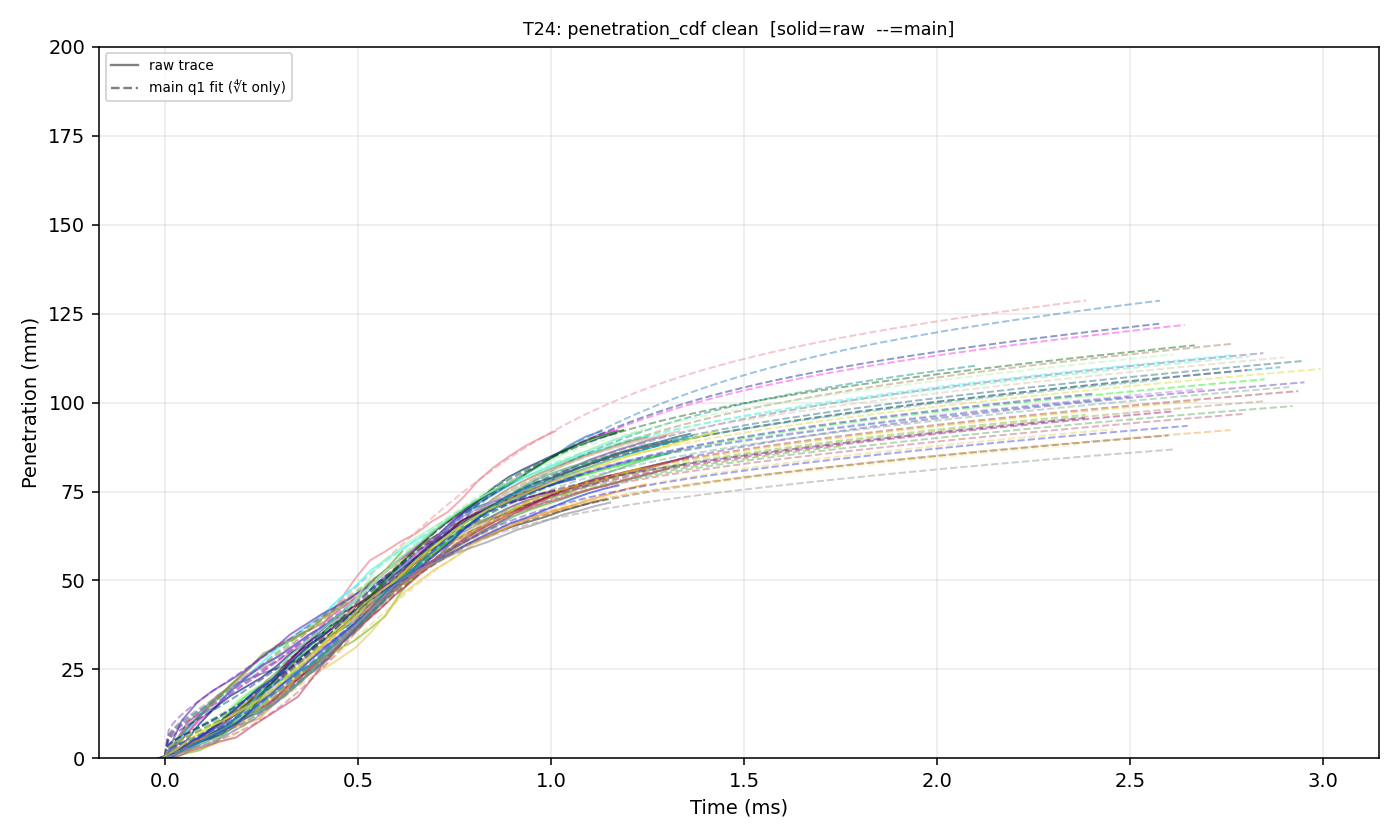
\includegraphics[width=0.92\linewidth]{images/representative_clean_fit.png}
\caption{Nozzle~1 上 T24 工况的清洗后轨迹与 q1 拟合曲线（\textbf{清洗后的 CDF 贯穿距离}）。实线表示逐帧原始贯穿距离观测，虚线为对应的 $t^{1/4}$ 单分支（q1）拟合曲线。拟合曲线在观测结束后平滑外推至 $\SI{3}{ms}$，为 surrogate 训练提供具备删失感知能力的目标。}
\label{fig:clean-fit-example}
\end{figure}

\FloatBarrier

\subsection{论断到证据映射}

表~\ref{tab:results-claims-map} 保留了重构前结果章节的论断到证据映射，
以保证可追溯性：每行陈述一项不同的评估论断及其协议、预测目标、样本量、
种子数、比较模型和核心结论。固定表格行引用刷新的
评估 bundle；LONO、课程、KD 分片和筛查行保留
归档论文工件，与第五章采用的来源划分一致。

\begin{table}[p]
\centering
\scriptsize
\setlength{\tabcolsep}{3pt}
\renewcommand{\arraystretch}{1.2}
\begin{tabular}{@{}L{0.12\linewidth}L{0.15\linewidth}L{0.13\linewidth}L{0.12\linewidth}L{0.16\linewidth}L{0.24\linewidth}@{}}
\toprule
论断 & 协议与目标 & $n$（点数） & 种子 & 比较模型 & 核心结论 \\
\midrule
域内点精度 & 未删失 CDF（主要） & \num{540367}/种子 & 5（7, 17, 42, 99, 2024） & MLP、SVGP、HA、NS & MLP \SI{4.185}{mm}（覆盖率 0.888/\allowbreak0.990）；SVGP 点预测最佳，为 \SI{4.087}{mm}（0.717/\allowbreak0.946）；两者均远低于基线 \\
\addlinespace
含删失（补充） & Full-clean CDF，包含右删失 & \num{689162}（21.6\% 删失点） & MLP 5；SVGP seed-42 & MLP、SVGP、HA、NS & MLP \SI{4.584}{mm}；SVGP \SI{4.440}{mm}；相较 HA/\allowbreak NS 为 $-59/-56\%$ \\
\addlinespace
观测中位数检查 & P50-observed，工况级 & \num{4215} & MLP 5；SVGP seed-42 & SVGP、MLP & SVGP 以 \SI{2.516}{mm} 领先；MLP 为 \SI{2.831}{mm} \\
\addlinespace
拟合延续检查 & q1 延续网格 & \num{25245}（\num{21525} 个外推点） & MLP 5；SVGP seed-42 & SVGP、MLP & SVGP \SI{9.680}{mm}；MLP \SI{10.047}{mm}；延续区域存在强正 bias \\
\addlinespace
喷嘴转移（完整） & LONO 5 折（留出 N0、N1、N2、N4、N5） & \num{458379} & seed-42 & MLP、SVGP；HA/\allowbreak NS 参考 & SVGP \SI{10.16}{mm} $<$ MLP \SI{12.55}{mm}；N0 折崩溃（34.76/\allowbreak26.99） \\
\addlinespace
设计族内转移（排除 N0） & LONO 4 折 & \num{147230} & seed-42 & MLP、SVGP & MLP \SI{7.00}{mm}，SVGP \SI{5.95}{mm}；覆盖率相互交织 \\
\addlinespace
课程消融 & LONO 5 折，分阶段流水线 & \num{458379}（5 折） & seed-42 & anchor / 区间变体 & $\mu$-anchor 教师 $+$ 不确定区间混合胜出；差距 $\ll$ CV 标准差 \\
\addlinespace
KD 形式修复 & 未删失 $+$ full-clean，5 种子 & \num{540367}/\allowbreak\num{692942}；分片 seed-99 & 5 & mixed-distill 对 forward-KL & 近 cap bias $-2.70\to-0.57$；RMSE \SI{4.185}{mm} 对种子稳健 \\
\addlinespace
Residual 后续 & 未删失 CDF；residual-LONO（训练中保留 N0） & \num{540367}；LONO \num{147013}（设计族内）/ \num{167771}（全部 5 折） & seed-42 & residual head/\allowbreak FiLM/\allowbreak SVGP 对已部署模型、SVGP & 可选域内后续为 \SI{3.921}{mm}（经 QC 重训练为 \SI{3.848}{mm}；\emph{未经} LONO 检验）；LONO 设计族内 $-31\%$（\SIrange{7.44}{5.16}{mm}） \\
\addlinespace
原型筛查演示 & 几何壁面接近筛查演示，玩具参数扫描（无实测真值） & 3 个设计变体 & n/a（单一已部署 checkpoint） & MLP（Stage~3，已部署） & 面向排名的几何分数（峰值 $P_{\mathrm{hit}}=77.66\%$，累积 $E$ 最高为 \SI{3.364}{ms}）；\emph{并非}经验证的撞壁概率 \\
\bottomrule
\end{tabular}
\caption{结果论断映射表，从重构前章节保留以保证论断可追溯性。每行是一项不同的评估论断，列出其协议、预测目标、样本量、种子数、比较模型和核心结论。固定表格行引用刷新的评估 bundle；LONO、课程、KD 分片和筛查行保留归档工件。不同协议的种子结构不同：生产表格使用 5 个种子（7/17/42/99/2024），所有 SVGP 行与 LONO/消融行使用单一种子（42），KD 区间分片表使用单一种子（99）。归档 bundle 还包含 oracle-q1 P50 下界（\SI{1.010}{mm}，不可部署），以及在外推 q1 网格中领先的诊断 KD 变体（\SI{10.358}{mm}）；这些模型不在刷新名册中，因此从本映射表中省略。}
\label{tab:results-claims-map}
\end{table}

\FloatBarrier

\subsection{生产 Surrogate 的刷新逐模型诊断}

下列图形是生产 MLP 在主要 QC-gated 未删失 CDF 表格上的刷新逐模型诊断，
由评估流水线重新生成。它们取代了支持重构前章节的
2026-05-21 归档逐模型诊断
（预测与测量散点图、residual 直方图、逐文件夹 RMSE、
逐种子 RMSE 和校准覆盖率审计）。以 Seed~99 作为代表性重复运行，
与早期章节的惯例一致。

\begin{figure}[t]
\centering
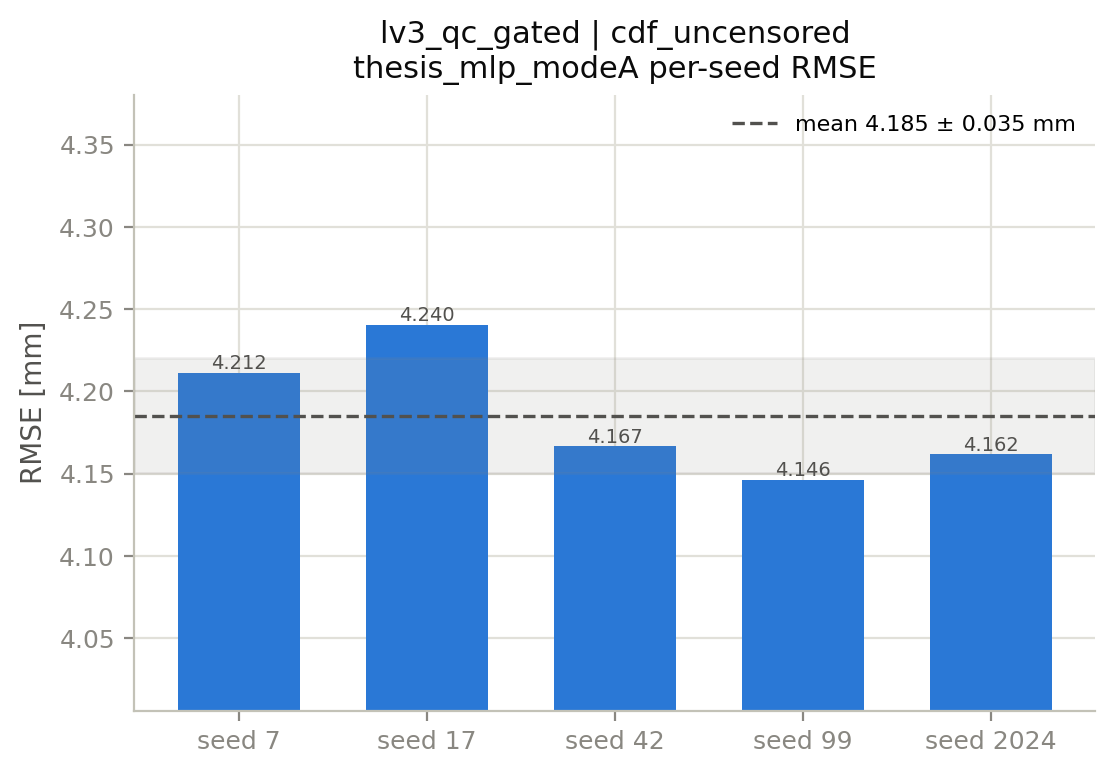
\includegraphics[width=0.80\linewidth]{images/eval_20260709/per_seed_rmse_thesis_mlp_modeA.png}
\caption{刷新后的 QC-gated 未删失 CDF 表格上五次生产训练重复运行（种子 7/17/42/99/2024）的逐种子 RMSE。}
\label{fig:app-per-seed-rmse}
\end{figure}

\begin{figure}[t]
\centering
\begin{minipage}{0.49\linewidth}
\centering
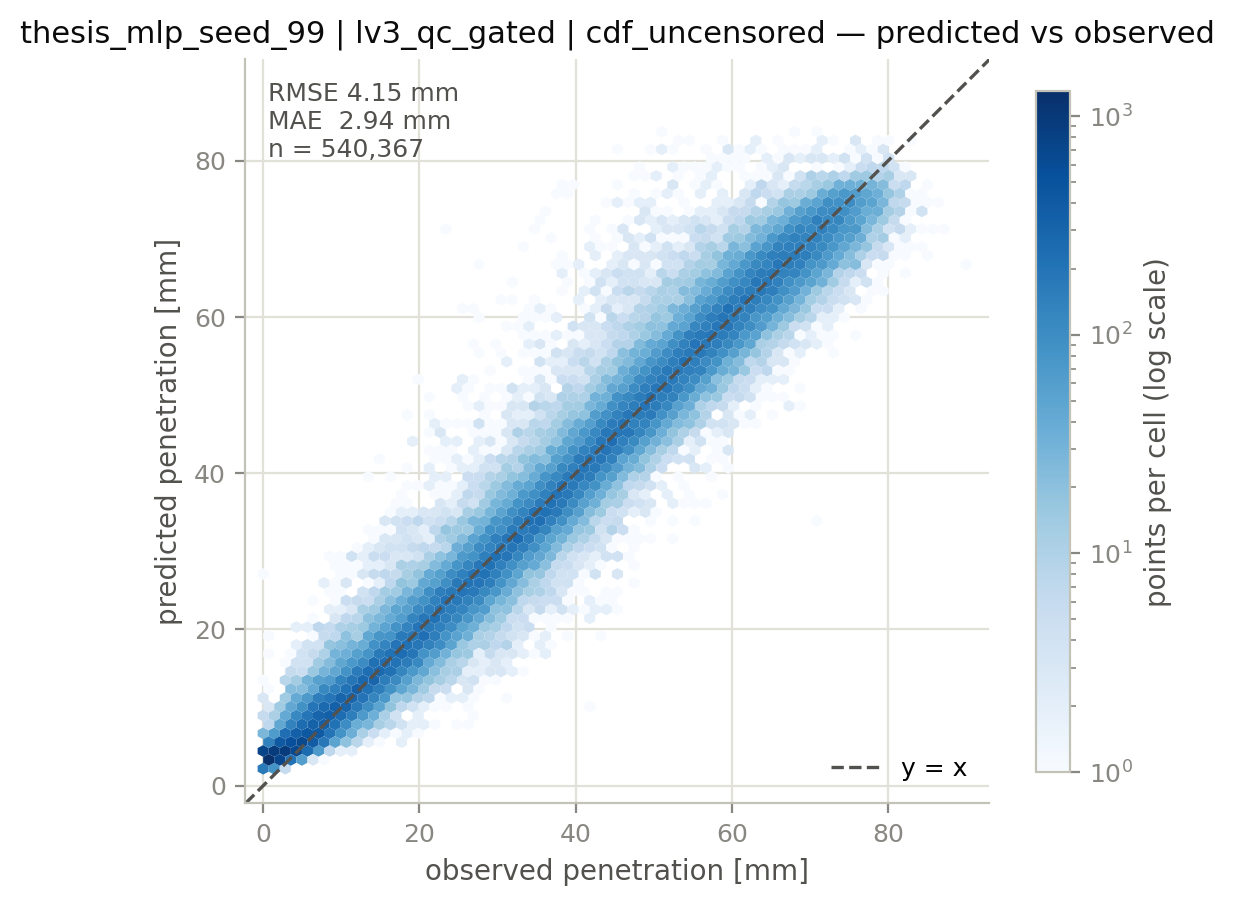
\includegraphics[width=\linewidth]{images/eval_20260709/mlp_seed99_pred_vs_actual.png}
\end{minipage}
\hfill
\begin{minipage}{0.49\linewidth}
\centering
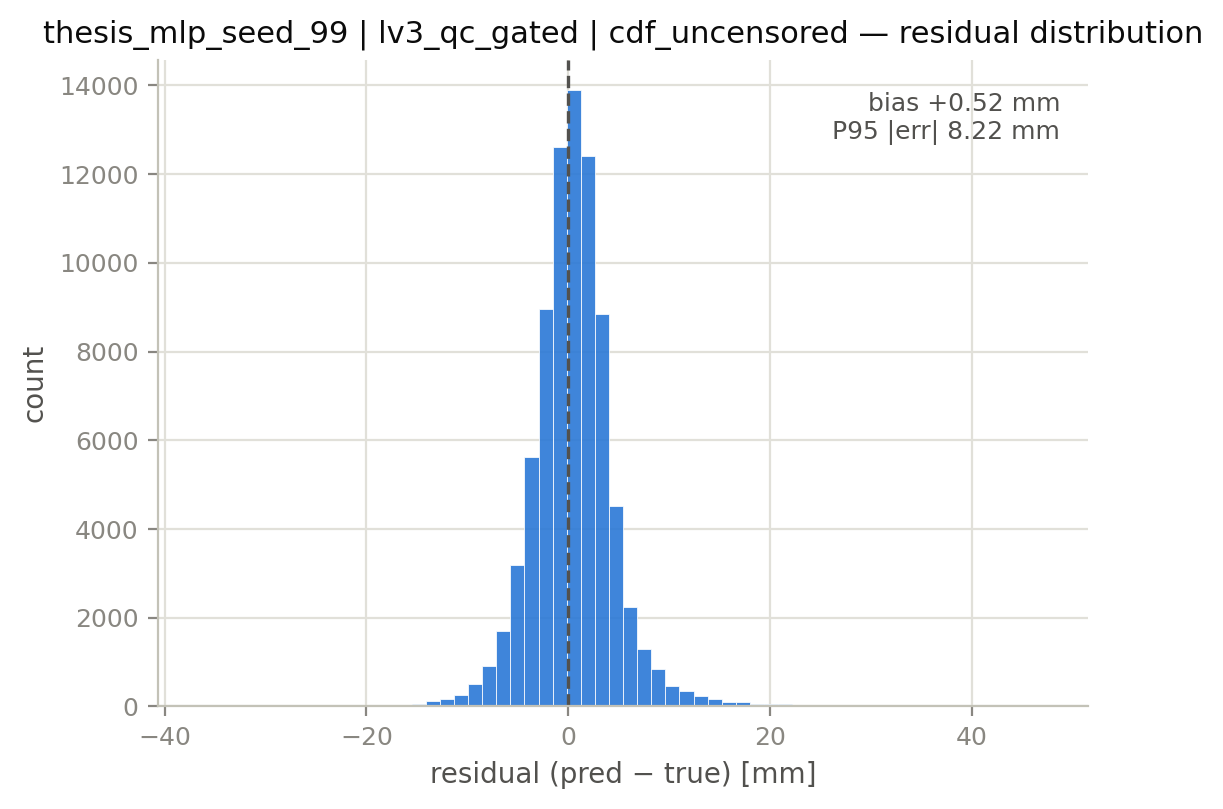
\includegraphics[width=\linewidth]{images/eval_20260709/mlp_seed99_residual_histogram.png}
\end{minipage}
\caption{刷新后的 QC-gated 未删失 CDF 表格上，代表性 seed-99 重复运行的预测与测量散点图（左）和 residual 直方图（右）。}
\label{fig:app-seed99-diagnostics}
\end{figure}

\begin{figure}[p]
\centering
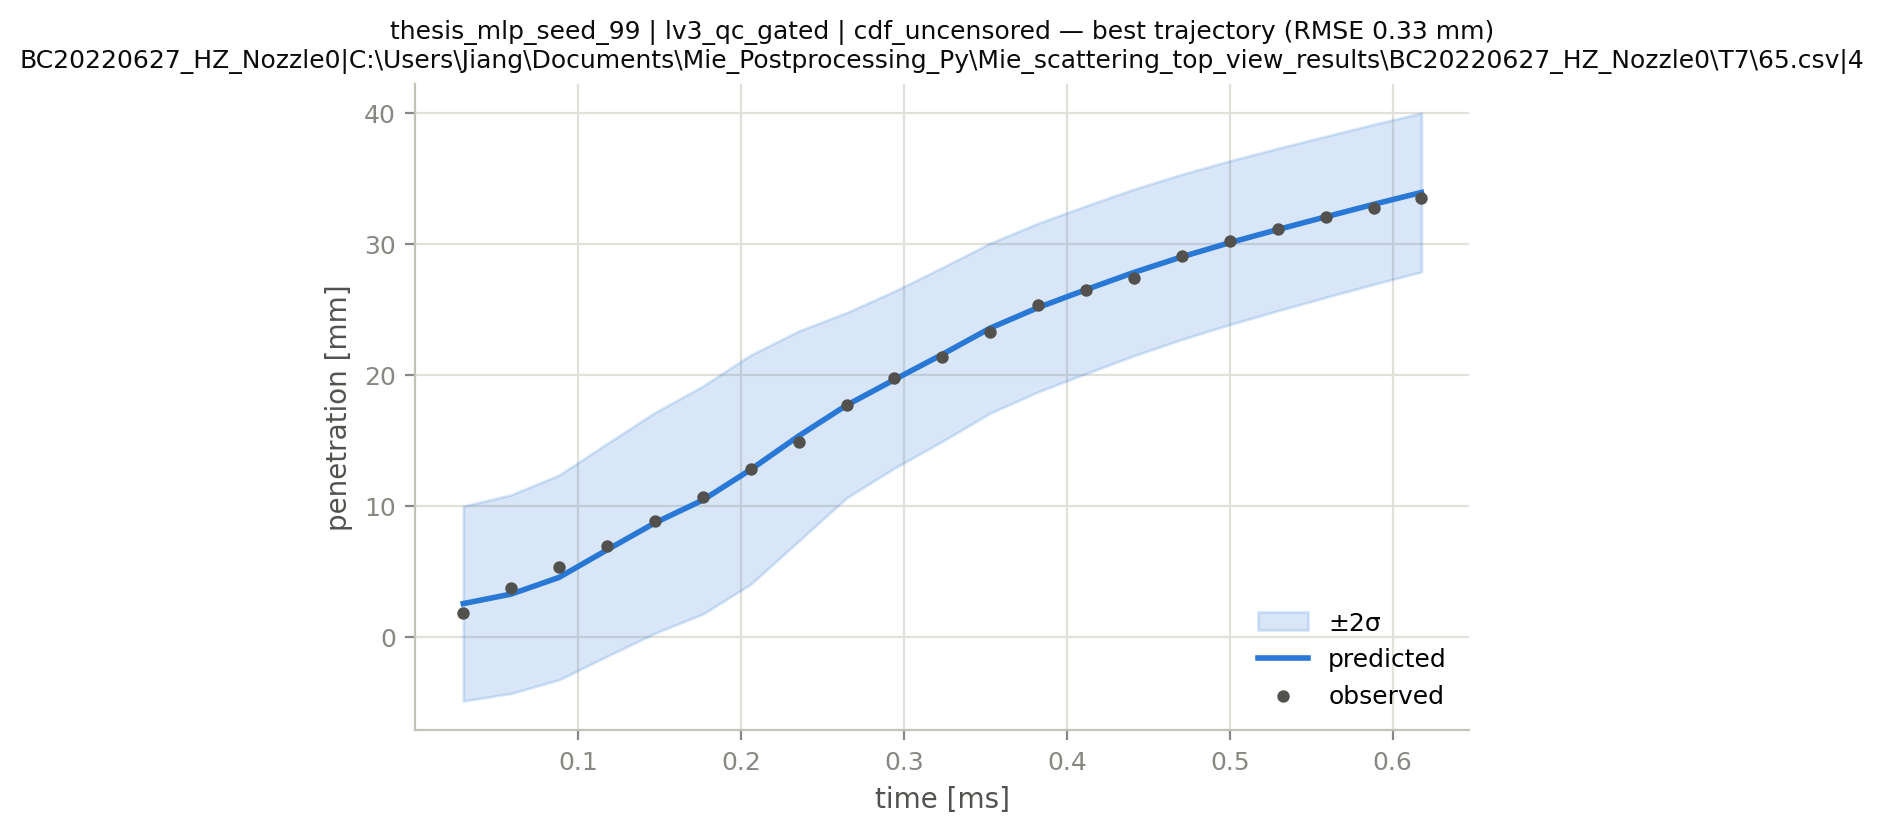
\includegraphics[width=0.94\linewidth]{images/eval_20260709/mlp_seed99_trajectory_best.png}\\[0.8em]
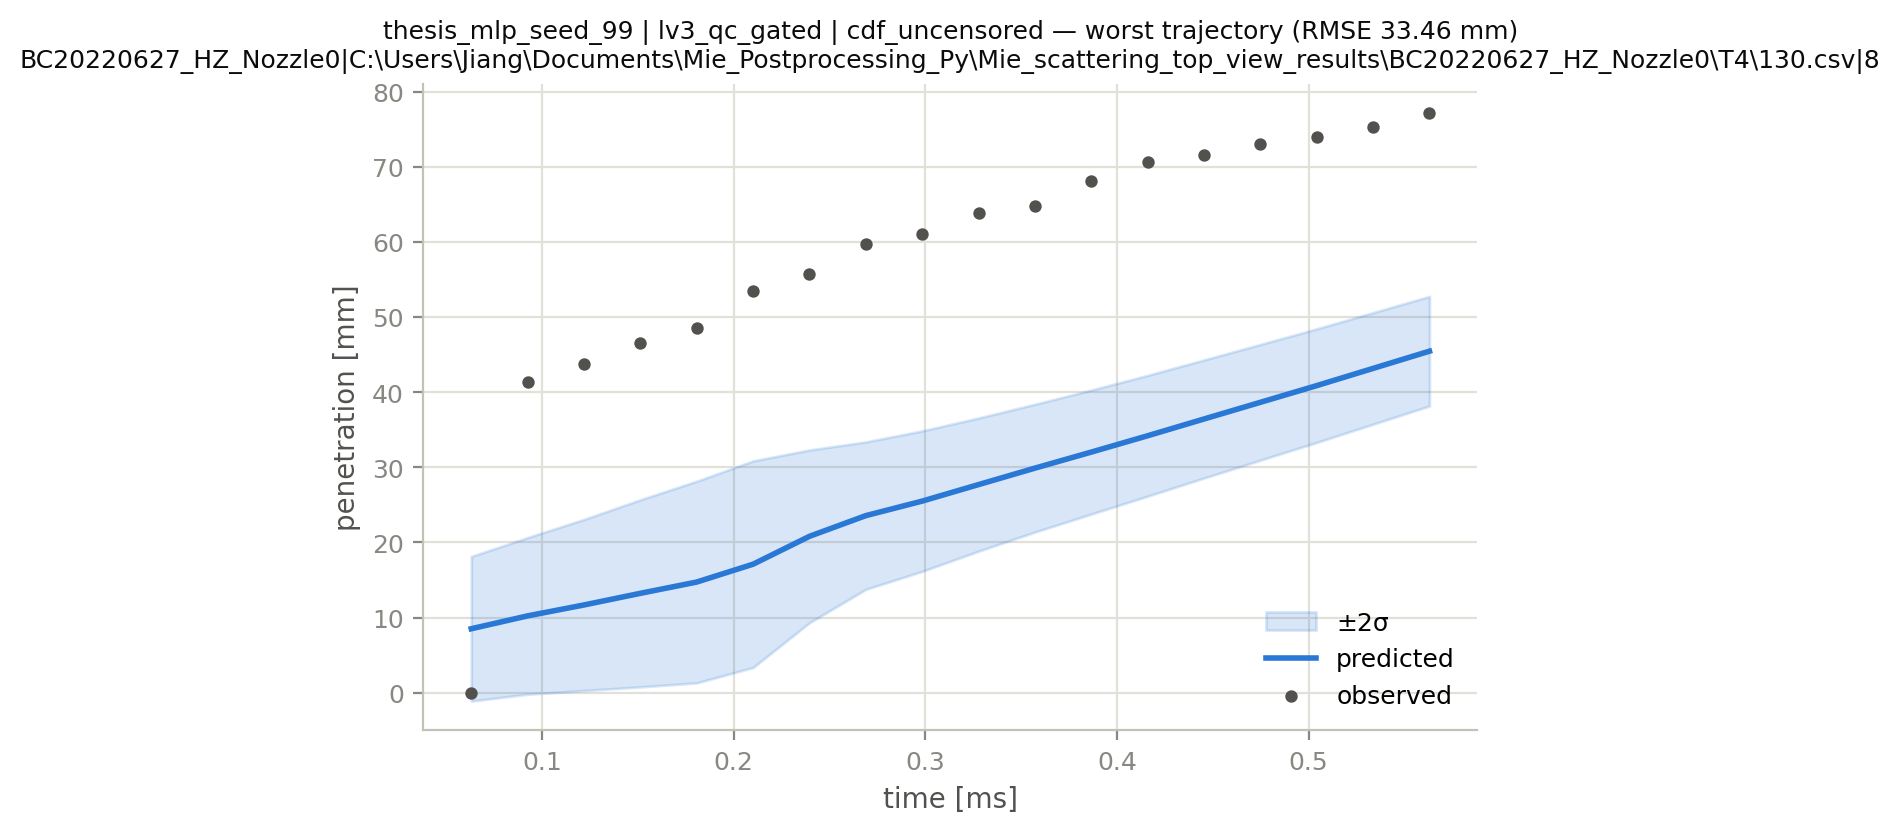
\includegraphics[width=0.94\linewidth]{images/eval_20260709/mlp_seed99_trajectory_worst.png}
\caption{刷新表格上 seed-99 重复运行自动选出的最佳拟合（上）和最差拟合（下）留出轨迹；选择准则为单条轨迹 RMSE 的最低值和最高值。最差案例重现了第五章 Nozzle-3 失效模式检查中讨论的瞬态形状失配。}
\label{fig:app-seed99-trajectories}
\end{figure}

\begin{figure}[t]
\centering
\begin{minipage}{0.49\linewidth}
\centering
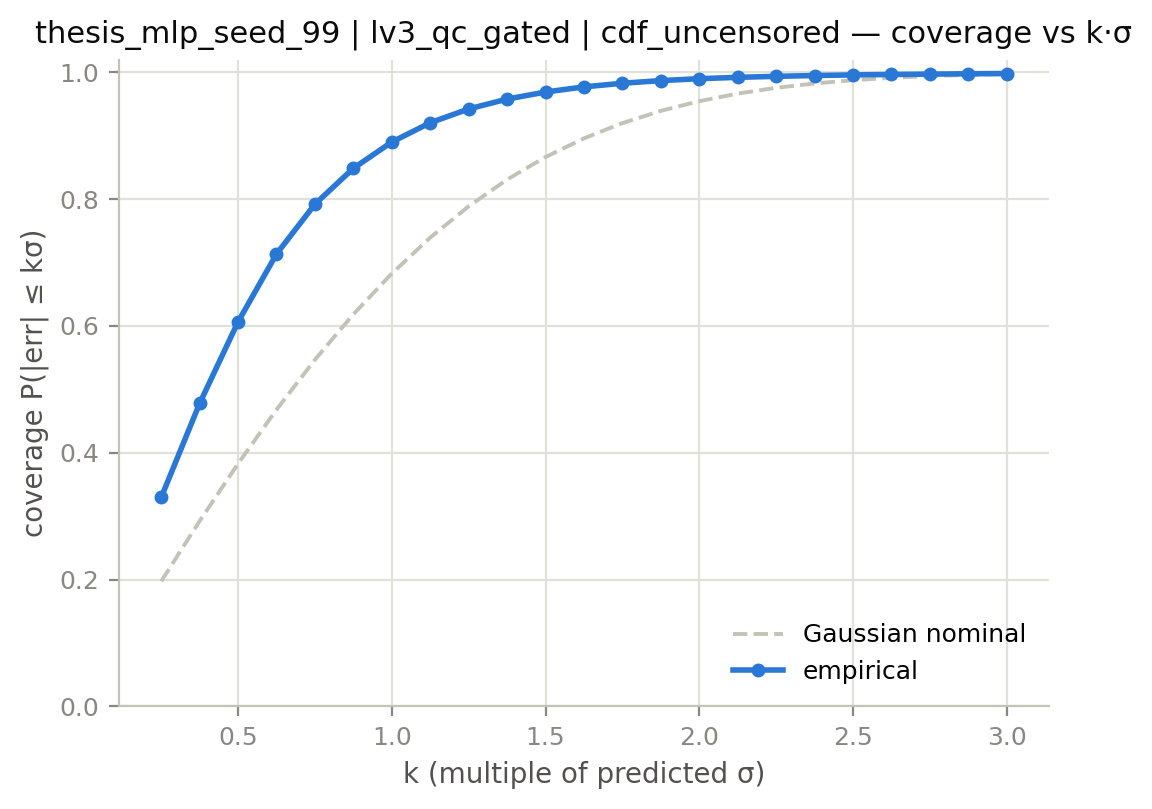
\includegraphics[width=\linewidth]{images/eval_20260709/mlp_seed99_coverage_curve.png}
\end{minipage}
\hfill
\begin{minipage}{0.49\linewidth}
\centering
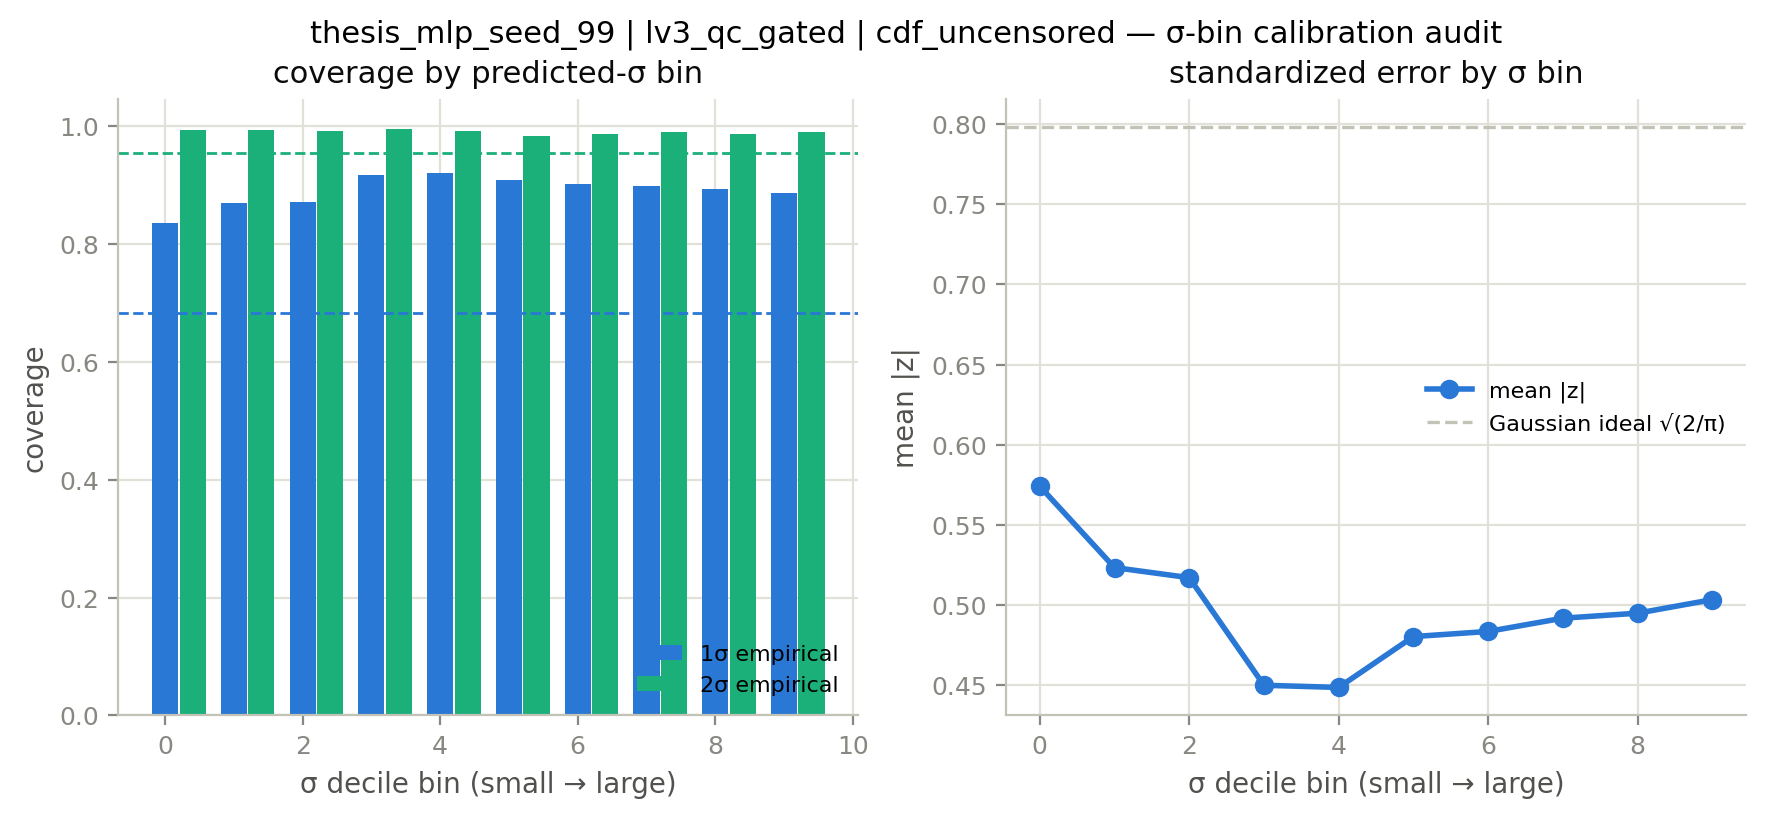
\includegraphics[width=\linewidth]{images/eval_20260709/mlp_seed99_sigma_bin_calibration.png}
\end{minipage}
\caption{seed-99 重复运行的刷新不确定度审计：经验覆盖率曲线（左）与按预测 $\sigma$ 分箱的校准（右）。二者取代了重构前章节的归档校准覆盖率审计。}
\label{fig:app-seed99-calibration}
\end{figure}

\begin{figure}[t]
\centering
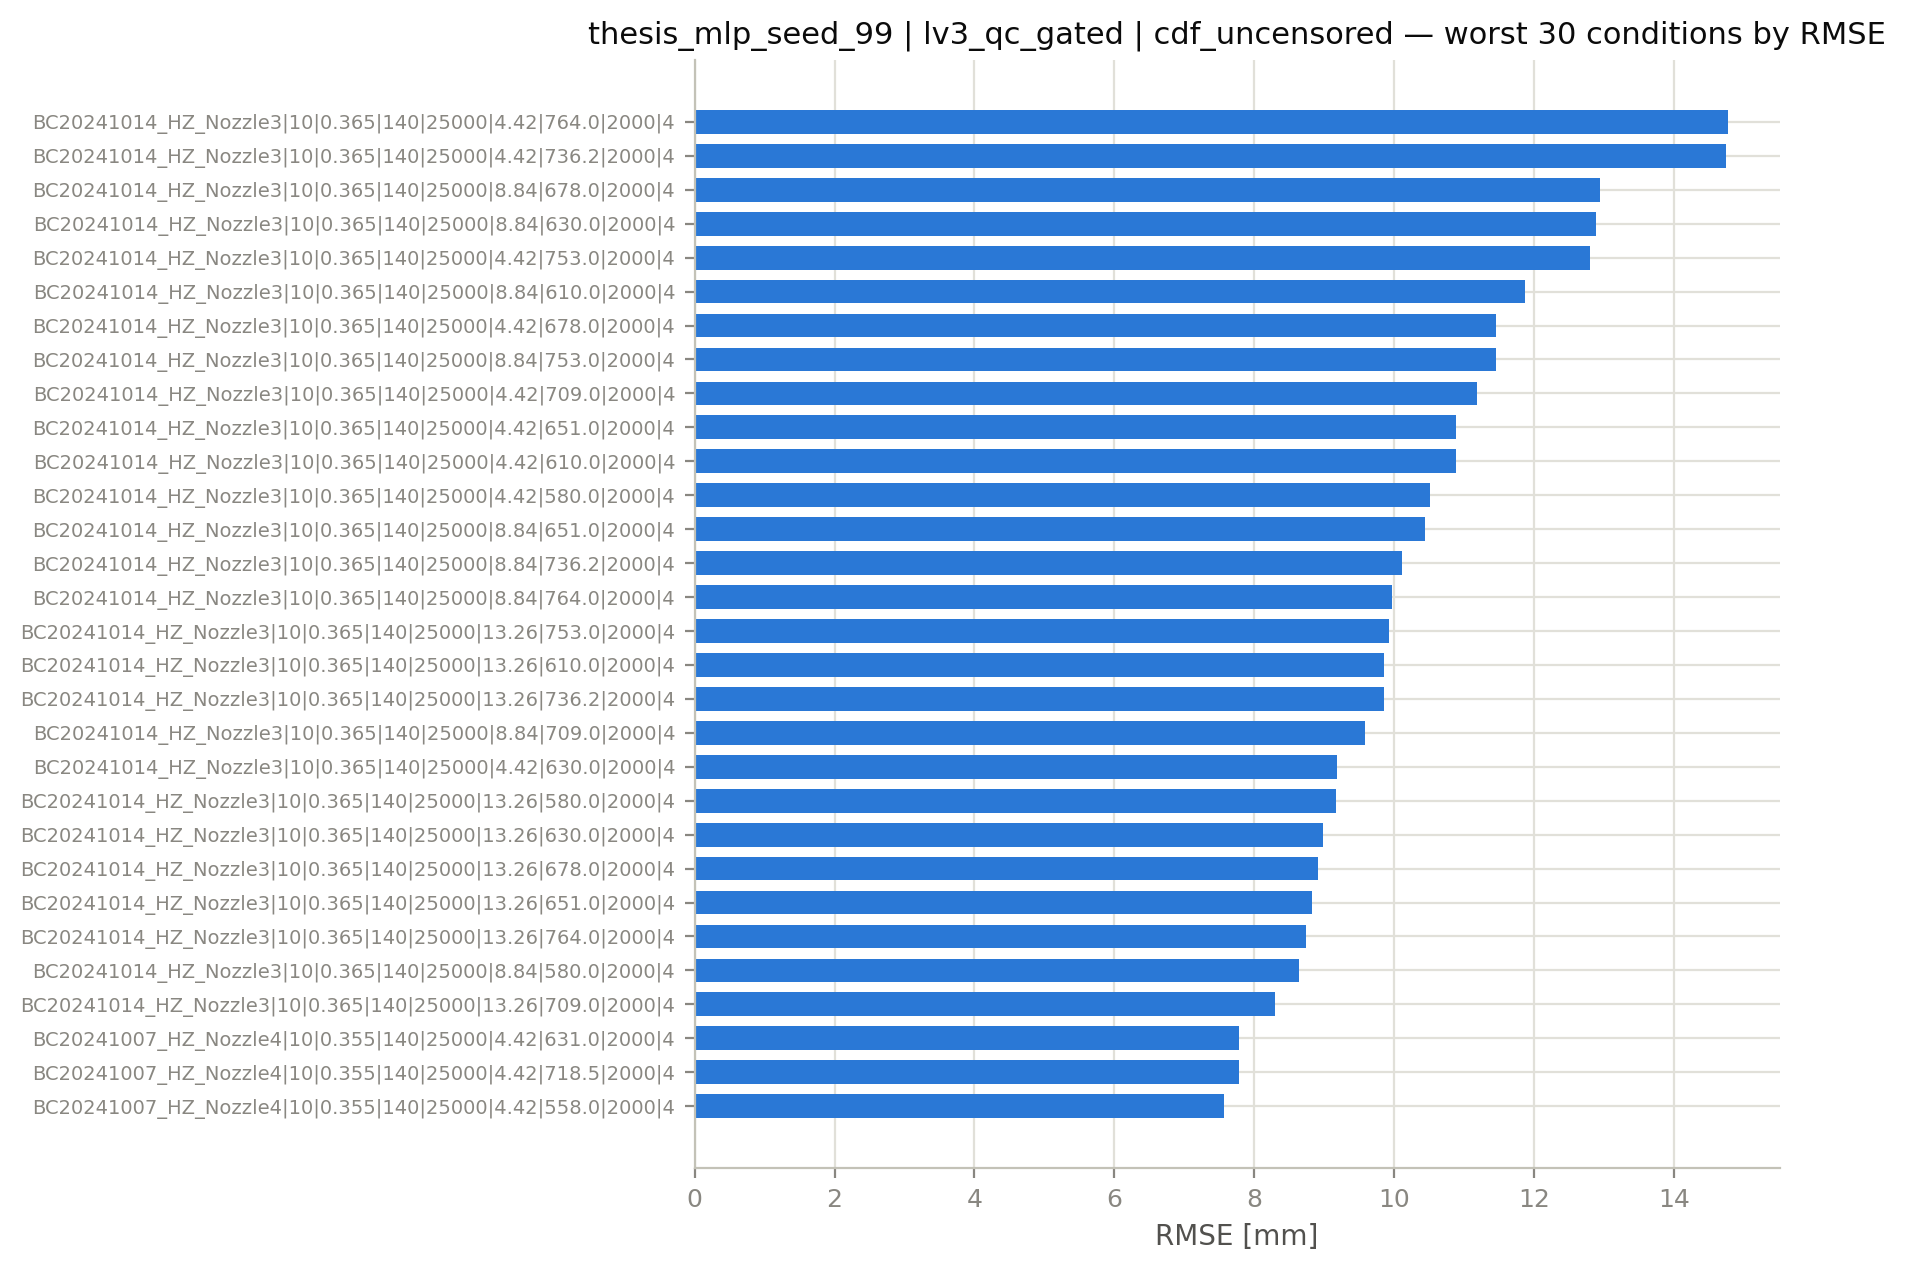
\includegraphics[width=0.88\linewidth]{images/eval_20260709/mlp_seed99_per_condition_rmse.png}
\caption{刷新后的 QC-gated 未删失 CDF 表格上 seed-99 重复运行的逐工况 RMSE，取代归档的逐文件夹 RMSE 诊断。误差在工况间仍呈不均匀分布，与重构前章节报告的 campaign 文件夹离散程度一致（最容易的文件夹处于较低的 \SI{3}{mm} 范围，最困难的接近 \SI{9}{mm}）。}
\label{fig:app-per-condition-rmse}
\end{figure}

\FloatBarrier

\subsection{课程消融细节（归档 LONO）}

下列表格保留了第五章压缩呈现的完整归档 LONO 消融证据：
带 bias 和覆盖率列的 Stage-2 anchor 调度比较、
其逐折明细，以及四变体 Stage-3 监督混合
排名。所有数值均为归档的单种子（42）五折 LONO 结果；
$\pm$ 项为跨折标准差。

\begin{table}[t]
\centering
\footnotesize
\setlength{\tabcolsep}{4pt}
\begin{tabular}{@{}L{0.30\linewidth}rrrr@{}}
\toprule
变体 & RMSE [mm] & MAE [mm] & Bias [mm] & 1$\sigma$ / 2$\sigma$ 覆盖率 \\
\midrule
\texttt{no\_anchor}        & 14.54 $\pm$ 12.36 & 10.80 $\pm$ \phantom{0}9.96 & $-8.50 \pm 11.03$ & 0.602 / 0.763 \\
\texttt{mu\_anchor}        & \textbf{12.73 $\pm$ 12.44} & \textbf{\phantom{0}9.86 $\pm$ 10.22} & \textbf{\boldmath$-7.11 \pm 11.51$} & 0.570 / \textbf{0.775} \\
\texttt{mu\_sigma\_anchor} & 13.05 $\pm$ 12.46 & 10.06 $\pm$ 10.33 & $-7.59 \pm 11.45$ & 0.564 / 0.764 \\
\bottomrule
\end{tabular}
\caption{Stage~2 anchor 调度 LONO 消融（归档）。每行报告 5 个留一喷嘴折（Nozzle0、Nozzle1、Nozzle2、Nozzle4、Nozzle5）的留出均值~$\pm$~标准差。选定的 Stage~2 教师配置为仅 $\mu$-anchor 变体，它同时在 RMSE、MAE、bias 绝对值和 2$\sigma$ 覆盖率上胜出。}
\label{tab:stage2-anchor-ablation}
\end{table}

\begin{table}[t]
\centering
\footnotesize
\setlength{\tabcolsep}{4pt}
\begin{tabular}{@{}L{0.28\linewidth}rrrrr|r@{}}
\toprule
变体 & Nozzle0 & Nozzle1 & Nozzle2 & Nozzle4 & Nozzle5 & 均值 \\
\midrule
\texttt{no\_anchor}        & 34.25 & \phantom{0}6.56 & 19.18 & 7.57 & 5.11 & 14.54 \\
\texttt{mu\_anchor}        & 34.92 & \phantom{0}7.16 & \textbf{\phantom{0}7.76} & 8.20 & 5.60 & \textbf{12.73} \\
\texttt{mu\_sigma\_anchor} & 35.12 & \phantom{0}7.10 & 10.04 & 7.73 & 5.27 & 13.05 \\
\bottomrule
\end{tabular}
\caption{三种 Stage~2 anchor 变体的逐折 LONO RMSE [mm]（归档）。三者均在 Nozzle0 折上失效（全新出厂的参考喷嘴，属于真正的跨设计族外推，且点数占主导）。产生区分的折为 Nozzle2；与仅 $\mu$-anchor 变体相比，省略 anchor 会使 RMSE 增加 \SI{11.4}{mm}。}
\label{tab:stage2-anchor-ablation-per-fold}
\end{table}

\begin{table}[t]
\centering
\footnotesize
\begin{tabular}{lrrrrr}
\toprule
配置 & RMSE [mm] & MAE [mm] & Bias [mm] & 1$\sigma$ 覆盖率 & 2$\sigma$ 覆盖率 \\
\midrule
基线配置 & 12.68 $\pm$ 12.74 & 9.97 $\pm$ 10.55 & $-7.86 \pm 11.28$ & 0.565 & 0.759 \\
仅可靠区间纯原始数据变体 & 12.76 $\pm$ 12.48 & 10.01 $\pm$ 10.22 & $-7.45 \pm 11.35$ & 0.556 & 0.761 \\
\textbf{不确定区间混合变体} & \textbf{12.55 $\pm$ 12.46} & \textbf{9.80 $\pm$ 10.18} & \textbf{\boldmath$-6.87 \pm 11.53$} & \textbf{0.575} & 0.770 \\
Anchor-off 变体 & 12.73 $\pm$ 12.44 & 9.86 $\pm$ 10.22 & $-7.11 \pm 11.51$ & 0.570 & \textbf{0.775} \\
\bottomrule
\end{tabular}
\caption{将 Stage~2 教师固定为仅 $\mu$-anchor 后的 Stage~3 LONO 消融（归档）。每行报告五个留一喷嘴折的留出均值~$\pm$~标准差。不确定区间混合变体在 RMSE/MAE 上胜出；anchor-off 变体表现出最强的 2$\sigma$ 覆盖率。Nozzle0 对每个变体而言仍是跨设计族失效（RMSE \SIrange{34.76}{35.31}{mm}，bias $\approx\SI{-27}{mm}$）。}
\label{tab:stage3-ablation-ranking}
\end{table}

\begin{figure}[t]
\centering
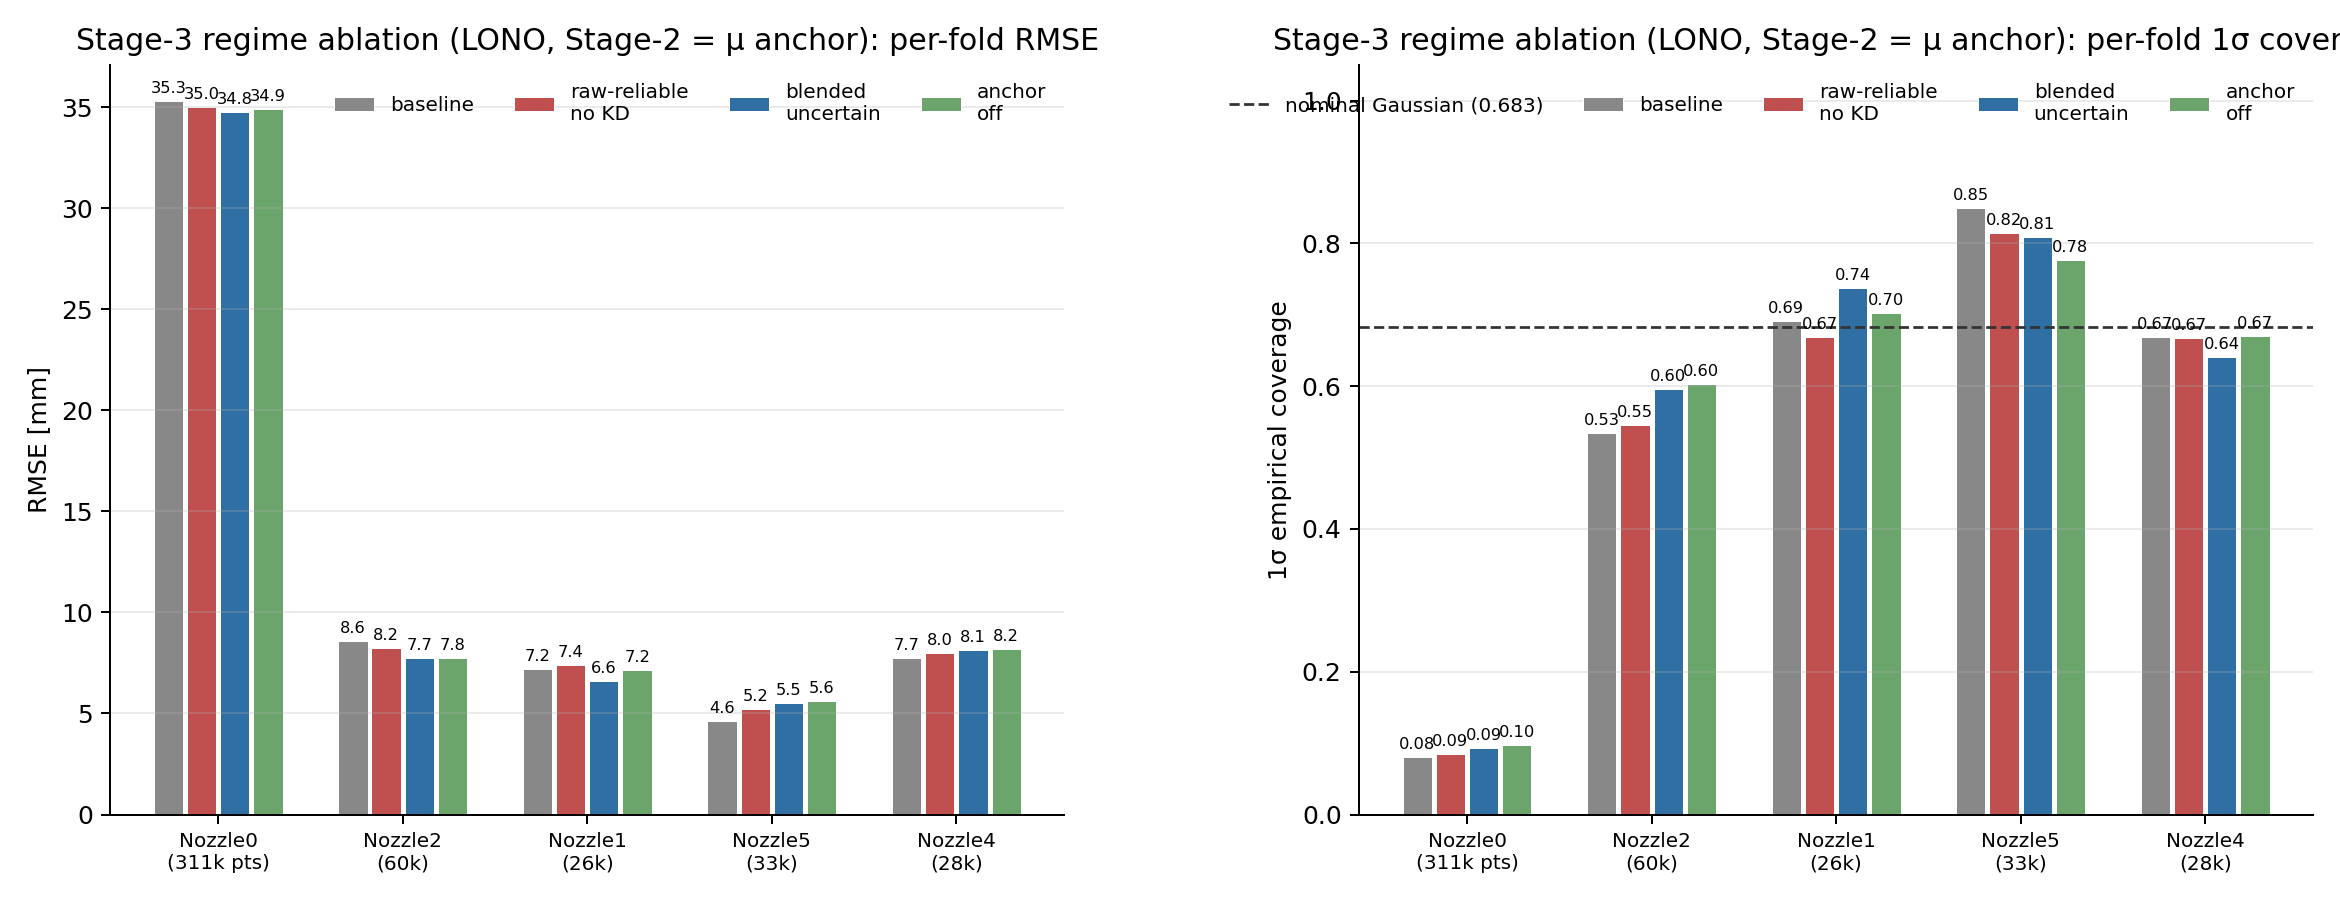
\includegraphics[width=\linewidth]{images/neural_network_fit_results/ablation_comparison_best.png}
\caption{归档 Stage~3 LONO 调优的汇总。将 Stage~2 教师固定为仅 $\mu$-anchor 后，不确定区间混合变体获得最低平均 RMSE/MAE，而 anchor-off 变体提供最强的 2$\sigma$ 覆盖率。源工件路径见附录~\ref{app:implementation_mapping}。}
\label{fig:ablation-best}
\end{figure}

\FloatBarrier

\subsection{KD 形式研究：监督区间与删失分片（归档）}

第五章报告了蒸馏损失修复的机制与核心结果。
归档的分片级证据保留于此。混合
蒸馏损失将均值 MSE 与对数方差 MSE 结合：
\begin{equation}
\mathcal{L}_{\mathrm{KD}} \;=\; (\mu_s-\mu_t)^{2} \;+\; \lambda_\sigma\,\bigl(\log\sigma_s^{2} - \log\sigma_t^{2}\bigr)^{2},
\label{eq:kd-mse-mu-plus-sigma}
\end{equation}
它显式重新监督 $\sigma$，同时消除 forward-KL 形式所允许的
方差膨胀逃逸路径。
表~\ref{tab:stage3-kd-regimes} 按训练
监督区间和 FOV 删失标志，对单一代表性种子
（99）的留出指标进行拆分；这些分片是在归档的含删失数据集
（692{,}942 个点）上计算的，因此其 Full Set 行是区间分片诊断，
而非刷新后的核心结果。

\begin{table}[t]
\centering
\small
\begin{tabular}{lrrrr}
\toprule
分片 & n & RMSE [mm] & Bias [mm] & 中位数 \(|\sigma_s-\sigma_t|\) [mm] \\
\midrule
完整数据集 & 692{,}942 & 4.76 & +0.72 & 0.82 \\
可靠原始数据区间 & 549{,}299 & 4.68 & +0.67 & 1.00 \\
不确定原始数据区间 & 64{,}487 & 5.88 & +1.27 & 0.40 \\
仅教师区间 & 79{,}156 & 4.33 & +0.65 & \textbf{0.27} \\
仅 KD（合并） & 143{,}643 & 5.08 & +0.93 & 0.32 \\
近 Cap（\(\mathrm{pen}\ge 0.9\,\mathrm{cap}\)） & 54{,}704 & 4.89 & \(-\)0.66 & 0.27 \\
轨迹未删失 & 393{,}912 & 4.85 & +0.99 & 0.81 \\
轨迹已删失 & 299{,}030 & 4.65 & +0.37 & 0.84 \\
轨迹已删失且近 Cap & 47{,}676 & 4.95 & \(-\)0.69 & 0.28 \\
\bottomrule
\end{tabular}
\caption{混合蒸馏模型（\(\lambda_\sigma=5.0\)，seed 99，归档含删失数据集）跨分片的归档留出指标。“可靠原始数据区间”表示由原始 NLL 主导的监督区；“仅 KD”合并不确定原始数据区间和仅教师区间，二者均通过式~\eqref{eq:kd-mse-mu-plus-sigma} 得到完全监督。中位数 \(|\sigma_s-\sigma_t|\) 逐点对比 Stage~2 教师的 \(\sigma\)，以量化校准漂移程度。}
\label{tab:stage3-kd-regimes}
\end{table}

\begin{figure}[t]
\centering
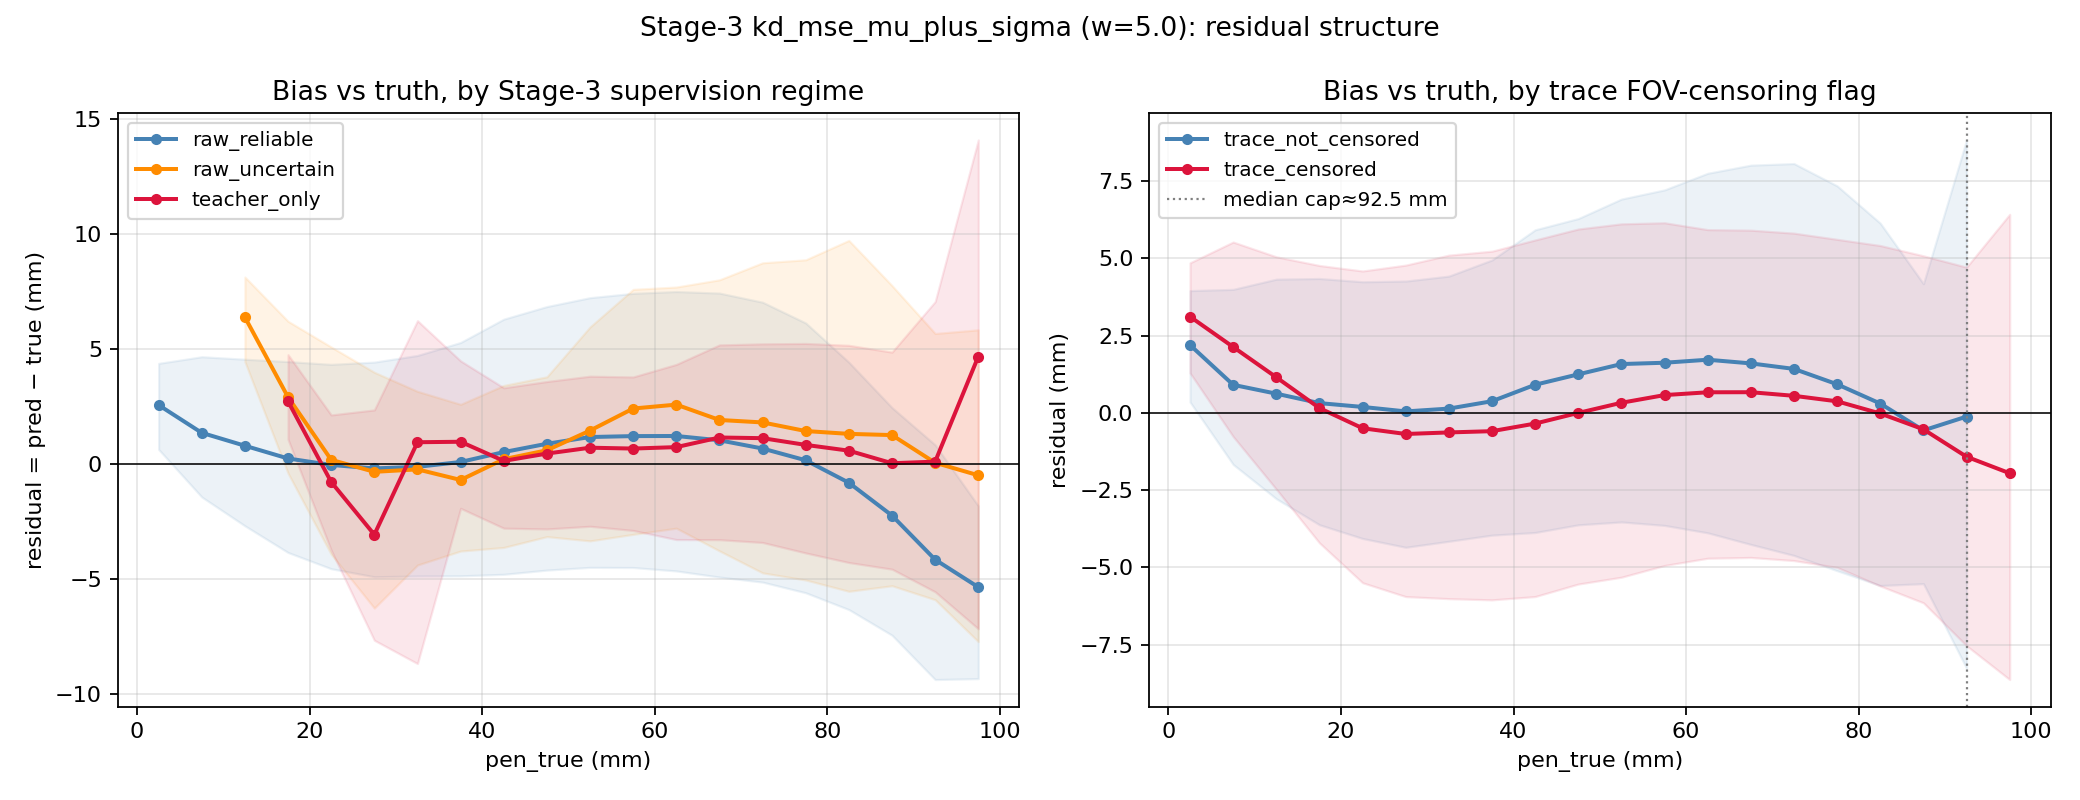
\includegraphics[width=\linewidth]{images/neural_network_fit_results/stage3_kd_mse_mu_plus_sigma_residual_vs_truth.png}
\caption{混合蒸馏模型（\(\lambda_\sigma=5\)）的归档 residual 结构。左：按训练区间分类（可靠原始数据 / 不确定原始数据 / 仅教师）。右：按轨迹级 FOV 删失标志分类。阴影区域对应 P10--P90 residual 范围。}
\label{fig:kd-residual-by-regime}
\end{figure}

\begin{figure}[t]
\centering
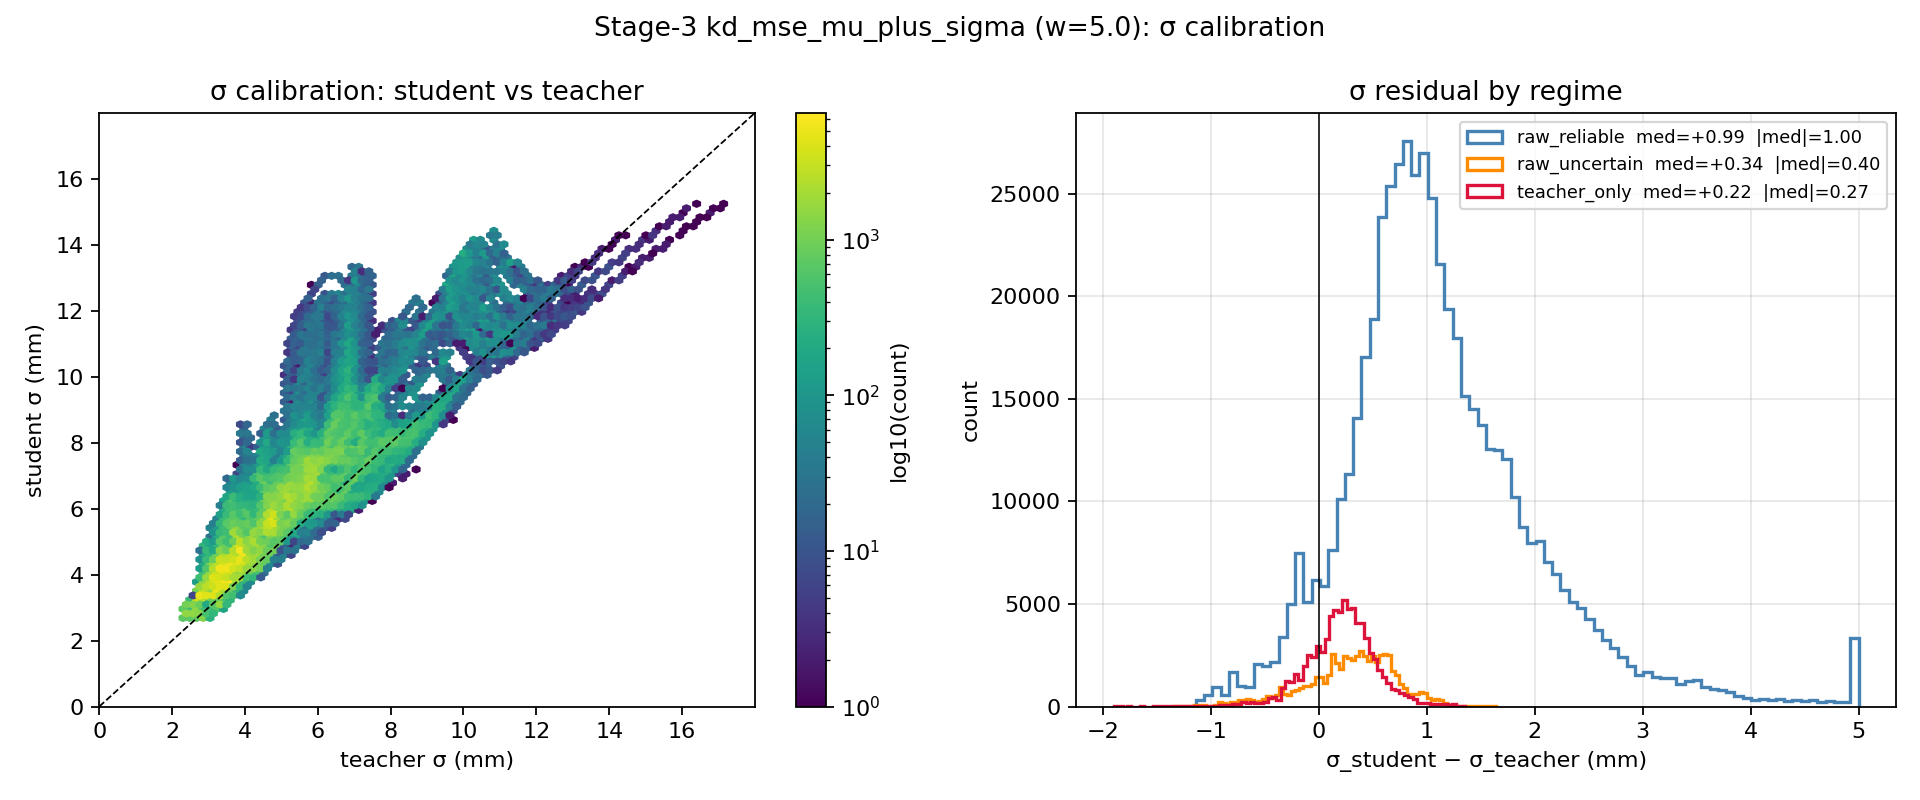
\includegraphics[width=\linewidth]{images/neural_network_fit_results/stage3_kd_mse_mu_plus_sigma_sigma_calibration.png}
\caption{混合蒸馏模型（\(\lambda_\sigma=5\)）的归档不确定度校准剖面。左：学生 \(\sigma\) 与教师 \(\sigma\) 的逐点 hex-bin 联合分布。右：不同监督区间中 residual \(\sigma_s-\sigma_t\) 的分布直方图。}
\label{fig:kd-sigma-calibration}
\end{figure}

\FloatBarrier

\subsection{Residual 适配细节}

下列两张表是第五章事后适配汇总背后的刷新细节：
喷油器 conditioning 设计比较，以及带校准列的完整
residual 逐步提升。二者均在 QC-gated
未删失 CDF 协议上重新生成；它们取代了原始研究
Level-2 时期的版本。后续图形归档自 2026-06-08
适配研究：其标注数值反映该研究的 Level-2 时期协议，
因此，当数值存在差异时，应以表格中的刷新结果为准。

% --- 刷新表格（来源：05_results_update_temp/appendix_fragments_residual.tex，已对照运行 20260709_223144 的 metrics_wide.csv 验证）---
\begin{table}[tbp]
\centering
\footnotesize
\setlength{\tabcolsep}{4pt}
\begin{tabular}{@{}L{0.32\linewidth}rrL{0.28\linewidth}@{}}
\toprule
喷油器 conditioning 设计 & RMSE [mm] & 95\% CI [mm] & 未见喷嘴的后备方案 \\
\midrule
One-hot 喷嘴输入（已部署；五种子均值） & 4.185 & --- & 无（需要硬编码身份） \\
独立逐喷嘴 head（\texttt{family\_head\_baseline}） & 4.901 & [4.845, 4.953] & 无（训练数据被分割） \\
Residual head，零初始化 $\Delta_f$（\texttt{residual\_fh}） & 4.519 & [4.463, 4.573] & 结构性后备（默认为共享模型） \\
\bottomrule
\end{tabular}
\caption{刷新后的 QC-gated 未删失 CDF 协议（540{,}367 个点）上的喷油器 conditioning 设计。数值来自 \texttt{evalrun\_\allowbreak{}20260709\_\allowbreak{}223144\_\allowbreak{}thesis\_\allowbreak{}full\_\allowbreak{}fullclean\_\allowbreak{}bootstrap\_\allowbreak{}fast\_\allowbreak{}20260709\_\allowbreak{}223142}；直接出现在 \texttt{metrics\_wide.csv} 中的单 checkpoint 设计显示 cluster-bootstrap 95\% 置信区间，而已部署结果是五种子生产 MLP 均值。}
\label{tab:residual-family-designs}
\end{table}

\begin{table}[tbp]
\centering
\footnotesize
\setlength{\tabcolsep}{3.5pt}
\begin{tabular}{@{}L{0.31\linewidth}rrrrrr@{}}
\toprule
模型 & RMSE & MAE & ECE & CRPS & P50 & 经 QC 重训练的 RMSE \\
\midrule
Naber--Siebers（参考） & 9.212 & 7.154 & --- & 5.109 & 8.983 & --- \\
生产 MLP，五种子均值（参考） & 4.185 & 2.978 & --- & 2.301 & 2.831 & --- \\
单输出 SVGP（参考） & 4.087 & 2.857 & 0.0214 & 2.063 & 2.516 & --- \\
\midrule
\texttt{family\_head\_baseline} & 4.901 & 3.518 & 0.0727 & 2.688 & 3.785 & --- \\
\texttt{residual\_fh} & 4.519 & 3.147 & 0.0612 & 2.351 & 3.264 & 4.590 \\
\texttt{residual\_film} & 4.401 & 3.035 & 0.0413 & 2.212 & 3.035 & 4.400 \\
\texttt{residual\_svgp} & \textbf{3.921} & \textbf{2.800} & \textbf{0.0267} & \textbf{2.019} & \textbf{2.026} & \textbf{3.848} \\
\bottomrule
\end{tabular}
\caption{来自 \texttt{evalrun\_\allowbreak{}20260709\_\allowbreak{}223144\_\allowbreak{}thesis\_\allowbreak{}full\_\allowbreak{}fullclean\_\allowbreak{}bootstrap\_\allowbreak{}fast\_\allowbreak{}20260709\_\allowbreak{}223142} 的刷新 \texttt{lv3\_qc\_gated} residual 模型逐步提升。RMSE、MAE、CRPS、P50 和经 QC 重训练的 RMSE 的单位为 mm；ECE 无量纲。CDF 指标使用 \texttt{cdf\_uncensored} 协议（540{,}367 个点），而 P50 是 \texttt{p50\_observed} 下的 RMSE（4{,}215 个点）；这些数值不得与早期 Level-2 表混用。Residual-SVGP 与经 QC 重训练的 residual-SVGP 变体未在匹配的 LONO 协议下评估。}
\label{tab:residual-climb}
\end{table}

\begin{figure}[t]
\centering
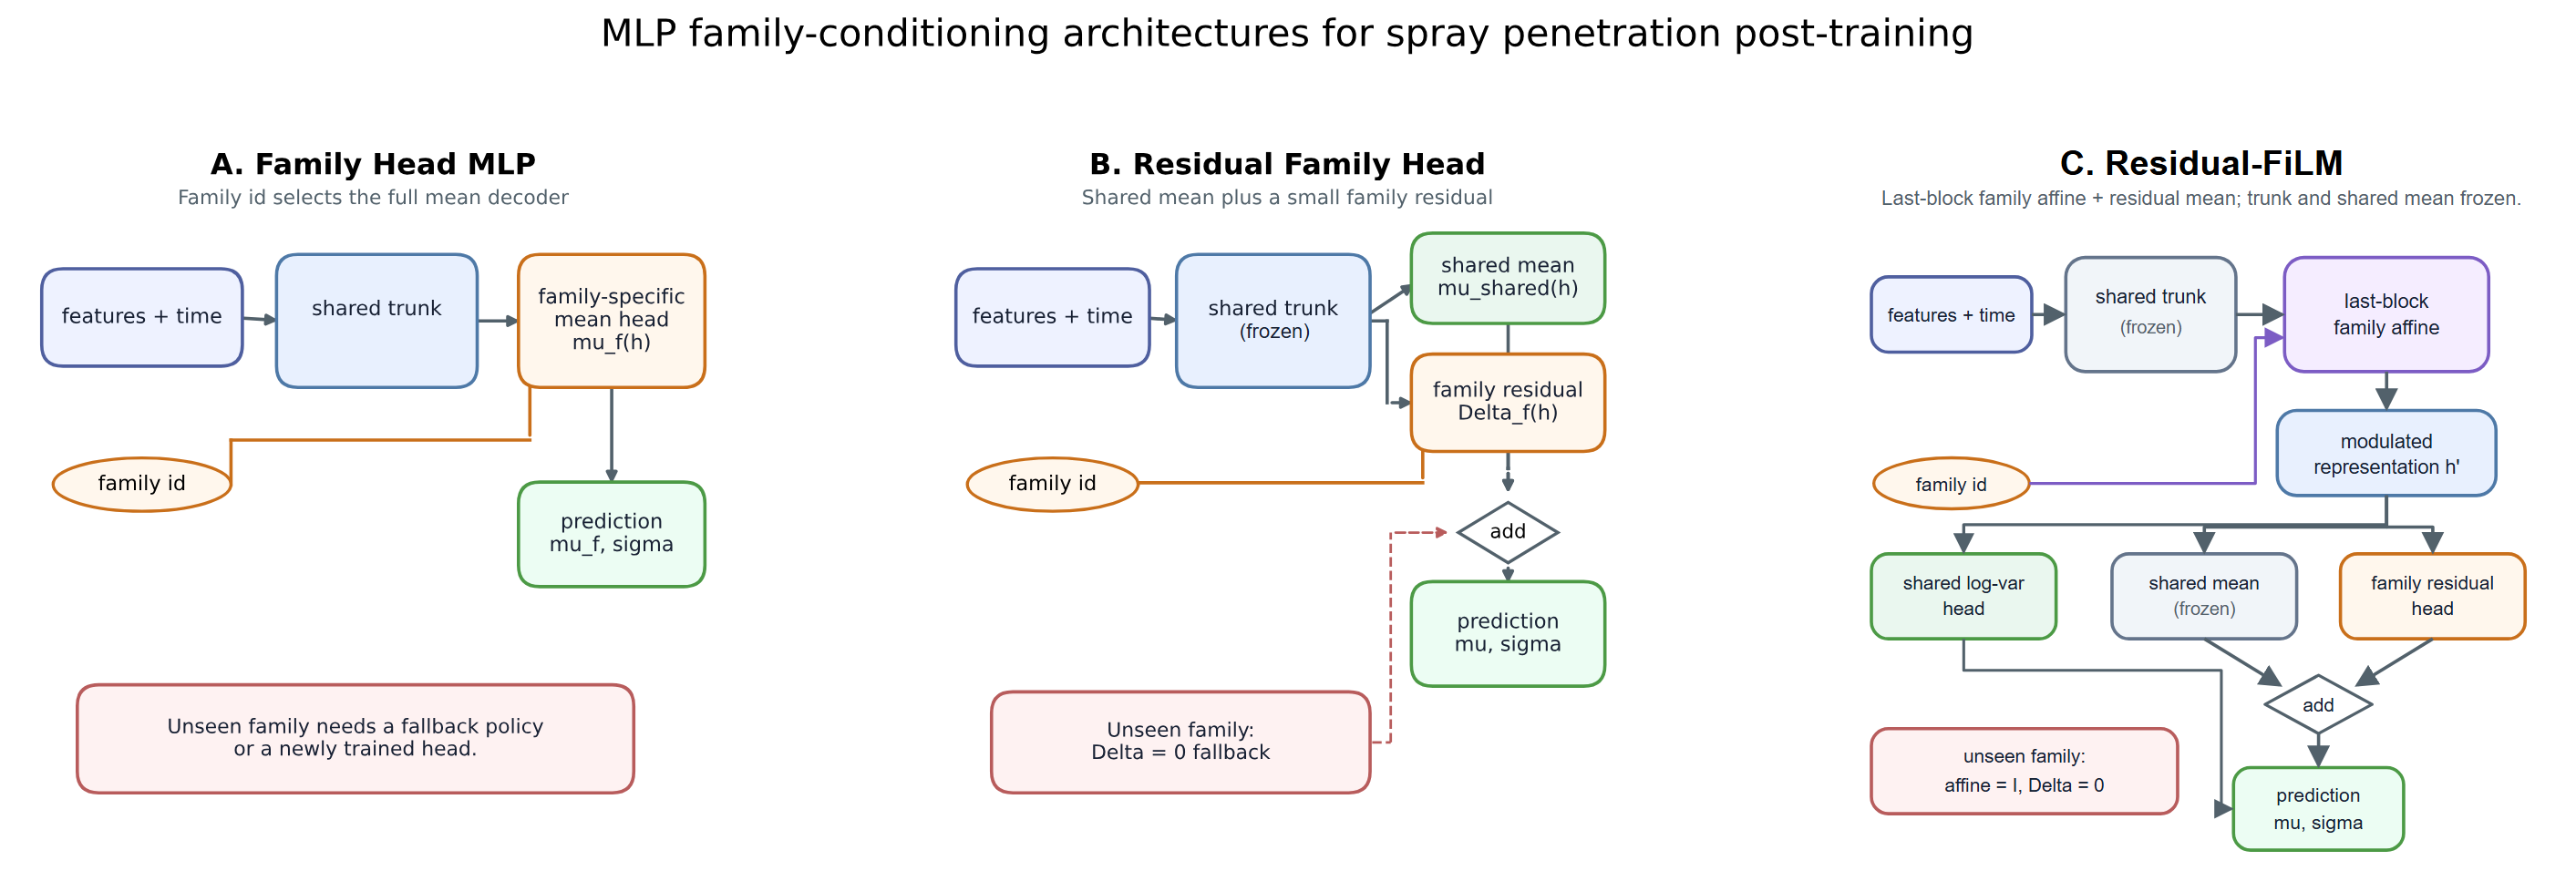
\includegraphics[width=0.96\linewidth]{images/residual_family_head_20260608/mlp_family_conditioning_architecture.png}
\caption{喷油器 conditioning 设计（归档研究）：独立逐喷嘴 head、加性 residual head 与 FiLM 调制。灰色 blocks 被冻结（从已部署 Stage~3 checkpoint 热启动）；绿色 blocks 是小型可训练逐喷嘴组件。}
\label{fig:residual-architecture}
\end{figure}

\begin{figure}[t]
\centering
\begin{minipage}{0.49\linewidth}
\centering
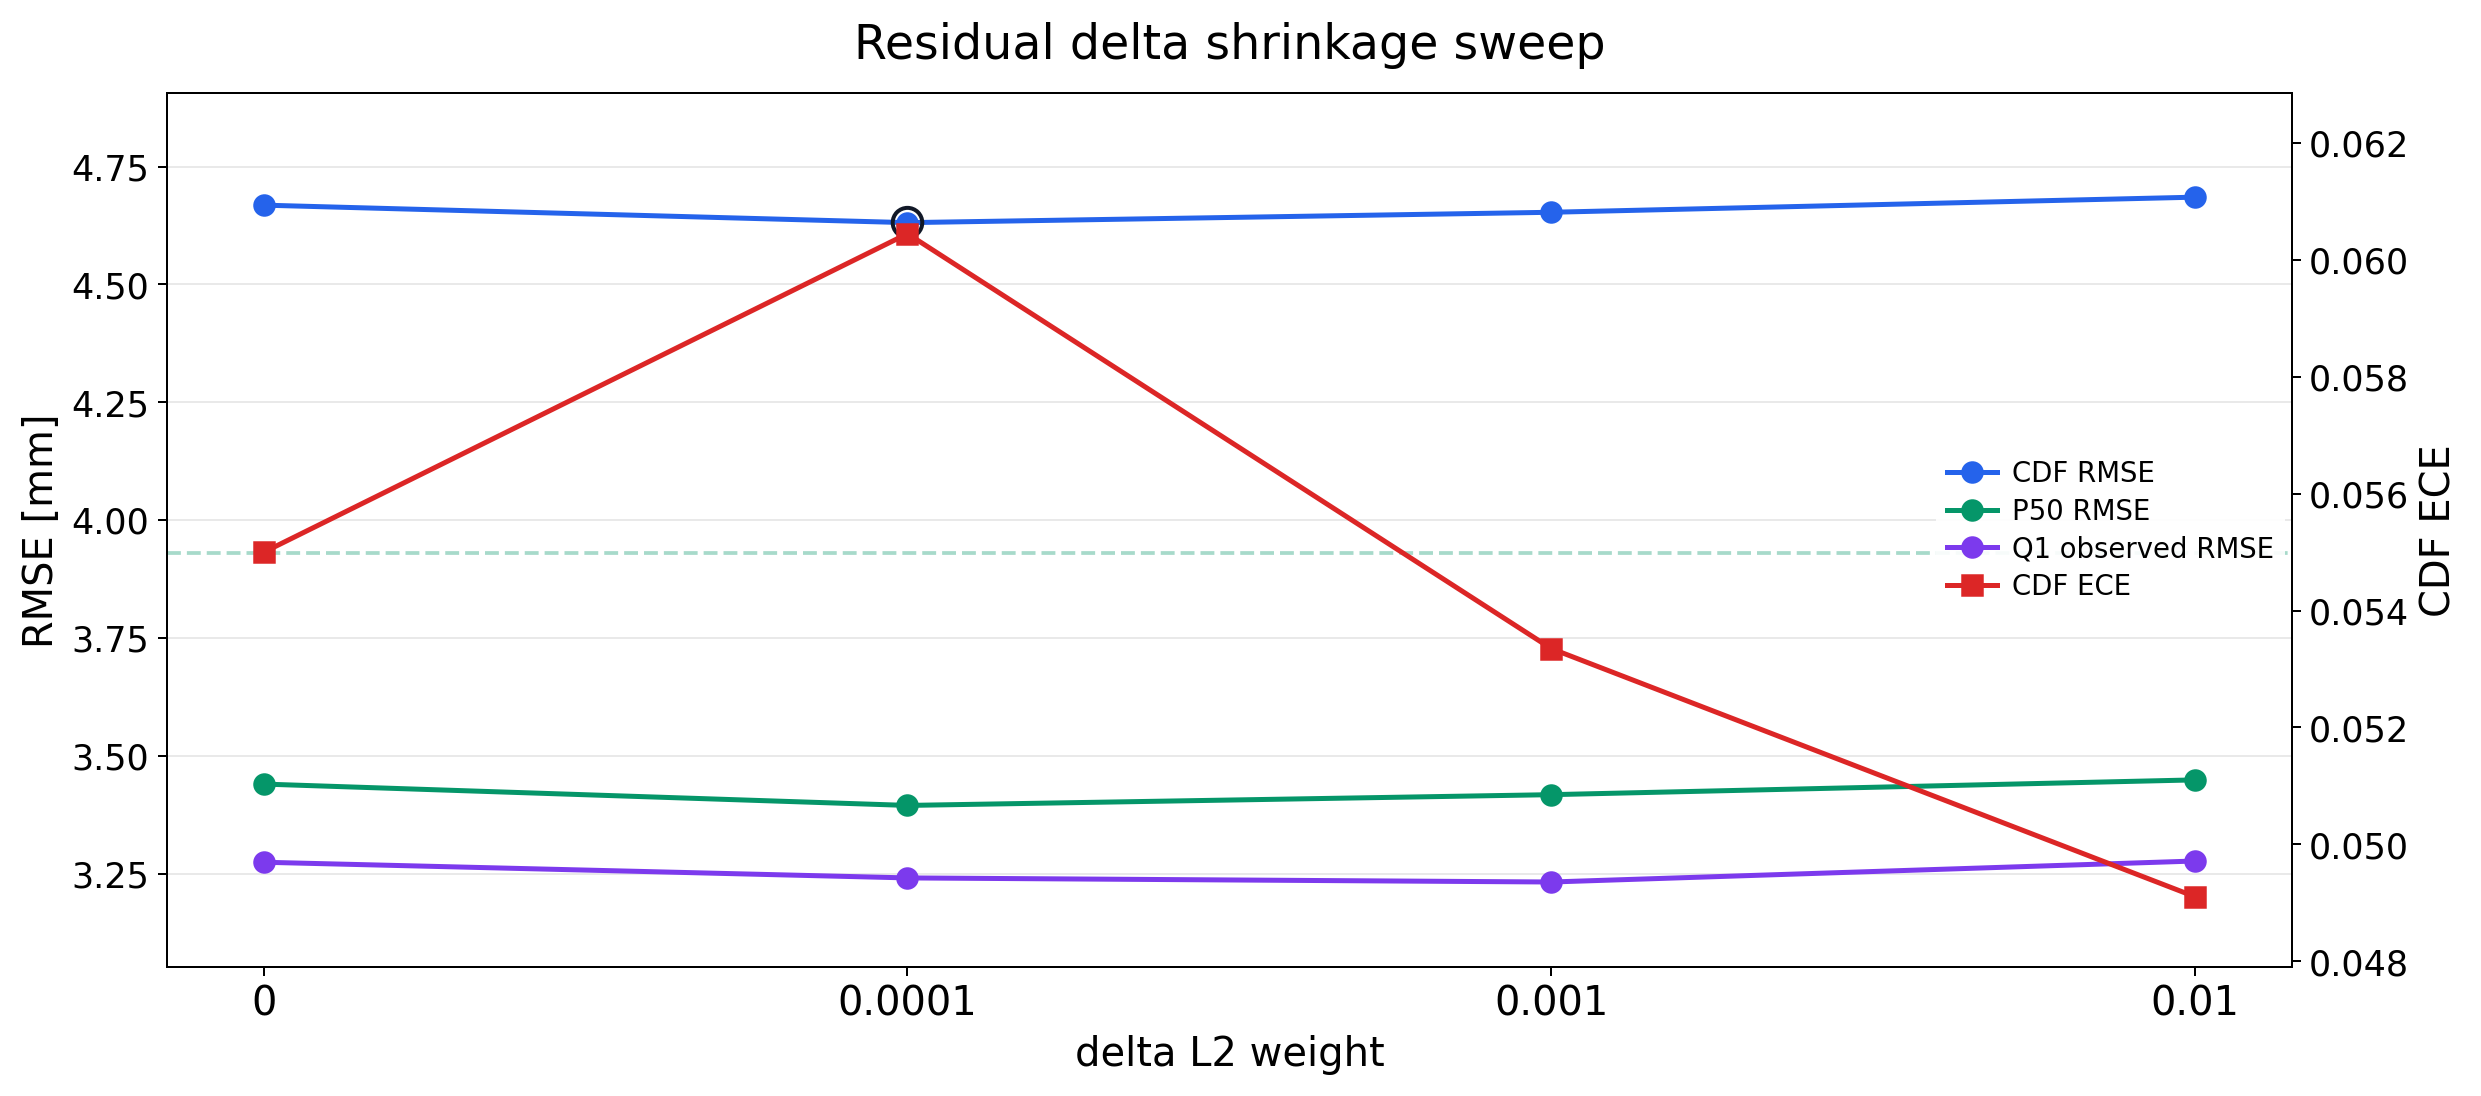
\includegraphics[width=\linewidth]{images/residual_family_head_20260608/delta_l2_sweep.png}
\end{minipage}
\hfill
\begin{minipage}{0.49\linewidth}
\centering
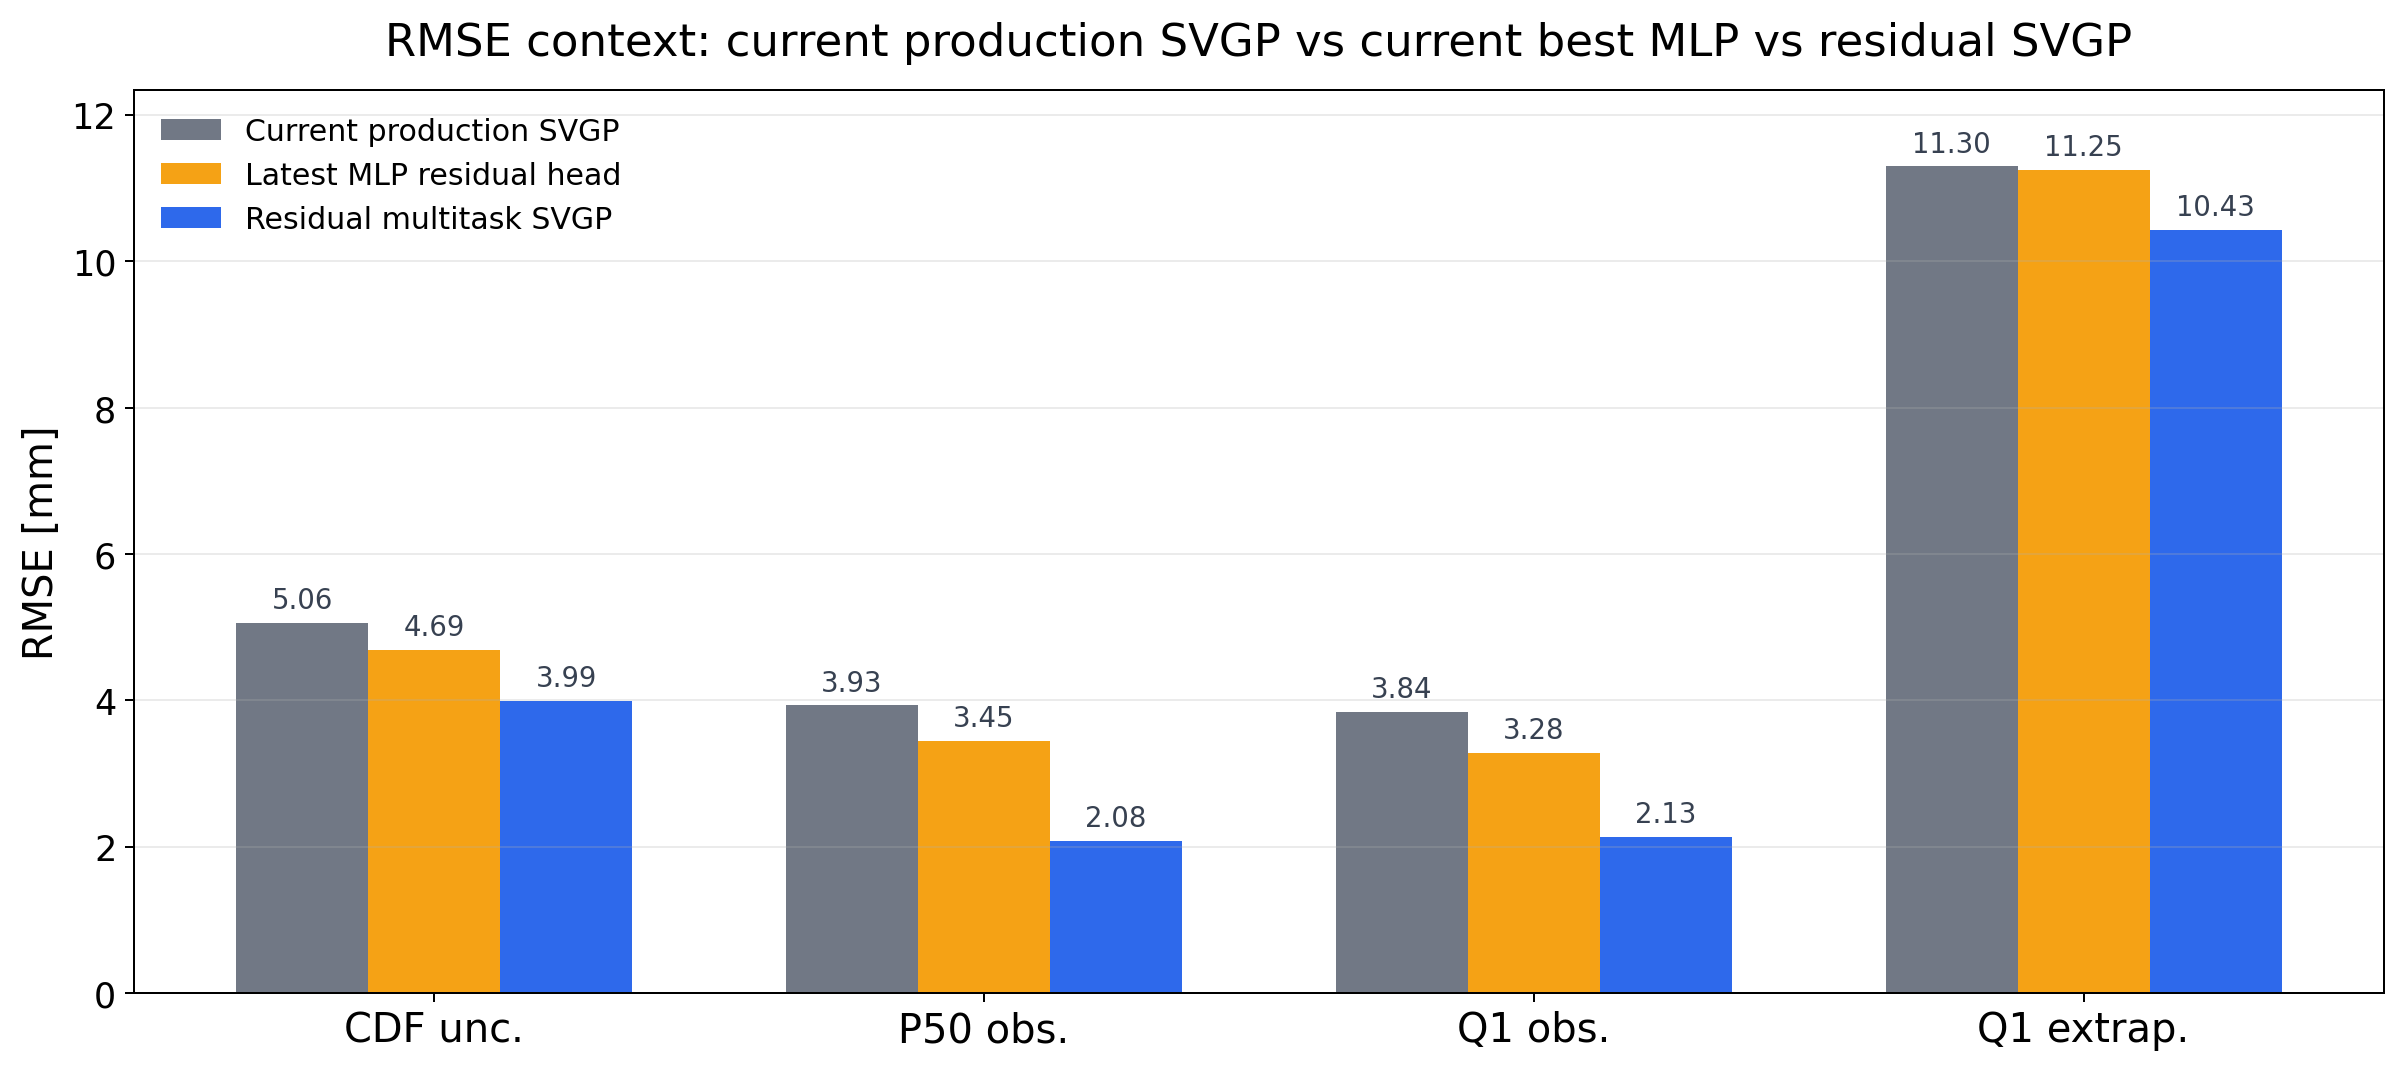
\includegraphics[width=\linewidth]{images/residual_family_head_20260608/residual_svgp_context_rmse_comparison.png}
\end{minipage}
\caption{归档适配研究诊断（Level-2 时期数值）。左：residual head 的收缩扫描（$\lambda_\Delta\in\{0,10^{-4},10^{-3},10^{-2}\}$）；每种设置均优于独立 head 后备方案。右：加性 residual multi-task SVGP 与同一表格上此前最佳结果的比较。刷新后的 QC-gated 数值见表~\ref{tab:residual-climb}。}
\label{fig:residual-svgp-climb}
\label{fig:residual-delta-sweep}
\end{figure}

\begin{table}[t]
\centering
\footnotesize
\begin{tabular}{@{}L{0.30\linewidth}rrr@{}}
\toprule
分支 & 设计族内 RMSE & 全部 5 折 RMSE & 设计族内 bias \\
 & （4 折，mm） & （5 折，mm） & （mm） \\
\midrule
已部署喷嘴 head & 7.44 $\pm$ 1.46 & 8.32 $\pm$ 2.33 & +5.07 \\
Residual head & \textbf{5.16 $\pm$ 0.65} & 6.95 $\pm$ 4.05 & +0.78 \\
Residual-FiLM & 5.15 $\pm$ 0.67 & 6.96 $\pm$ 4.08 & +0.75 \\
\bottomrule
\end{tabular}
\caption{MLP 分支上 residual 转换的归档 LONO 转移（依次留出 N1/N2/N4/N5/N6，训练中保留 N0，每折从头训练）。设计族内汇总排除了设计族之外的 N6 压力折。residual 转换将设计族内 RMSE 降低 $\approx$31\%，并修复均值 bias；FiLM 与普通 residual head 在转移下无法区分。}
\label{tab:residual-lono}
\end{table}

\begin{figure}[t]
\centering
\begin{minipage}{0.49\linewidth}
\centering
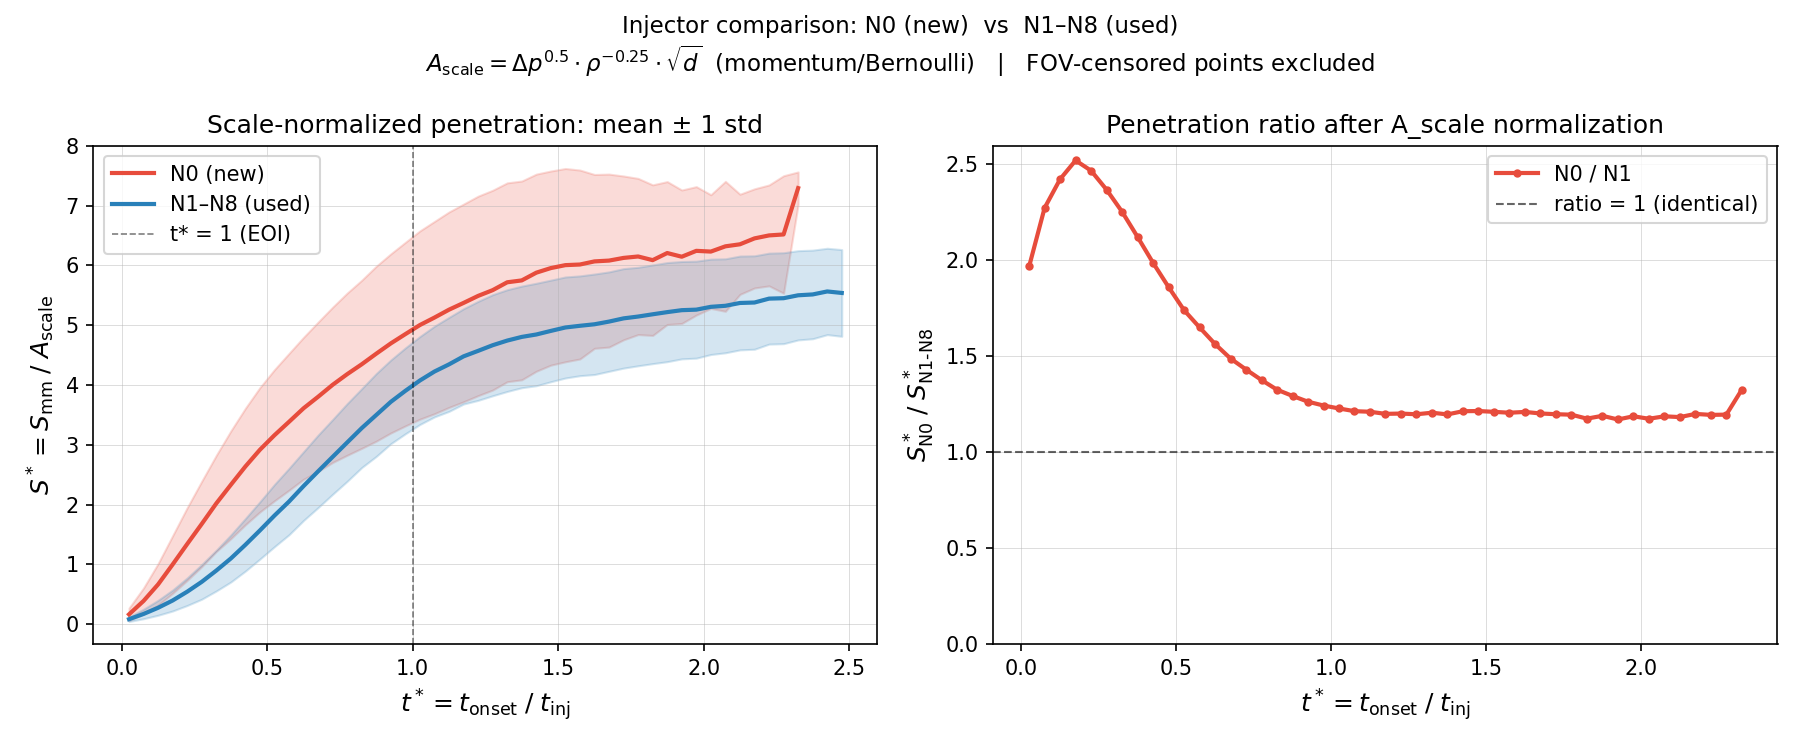
\includegraphics[width=\linewidth]{images/residual_family_head_20260608/injector_comparison_dp050.png}
\end{minipage}
\hfill
\begin{minipage}{0.49\linewidth}
\centering
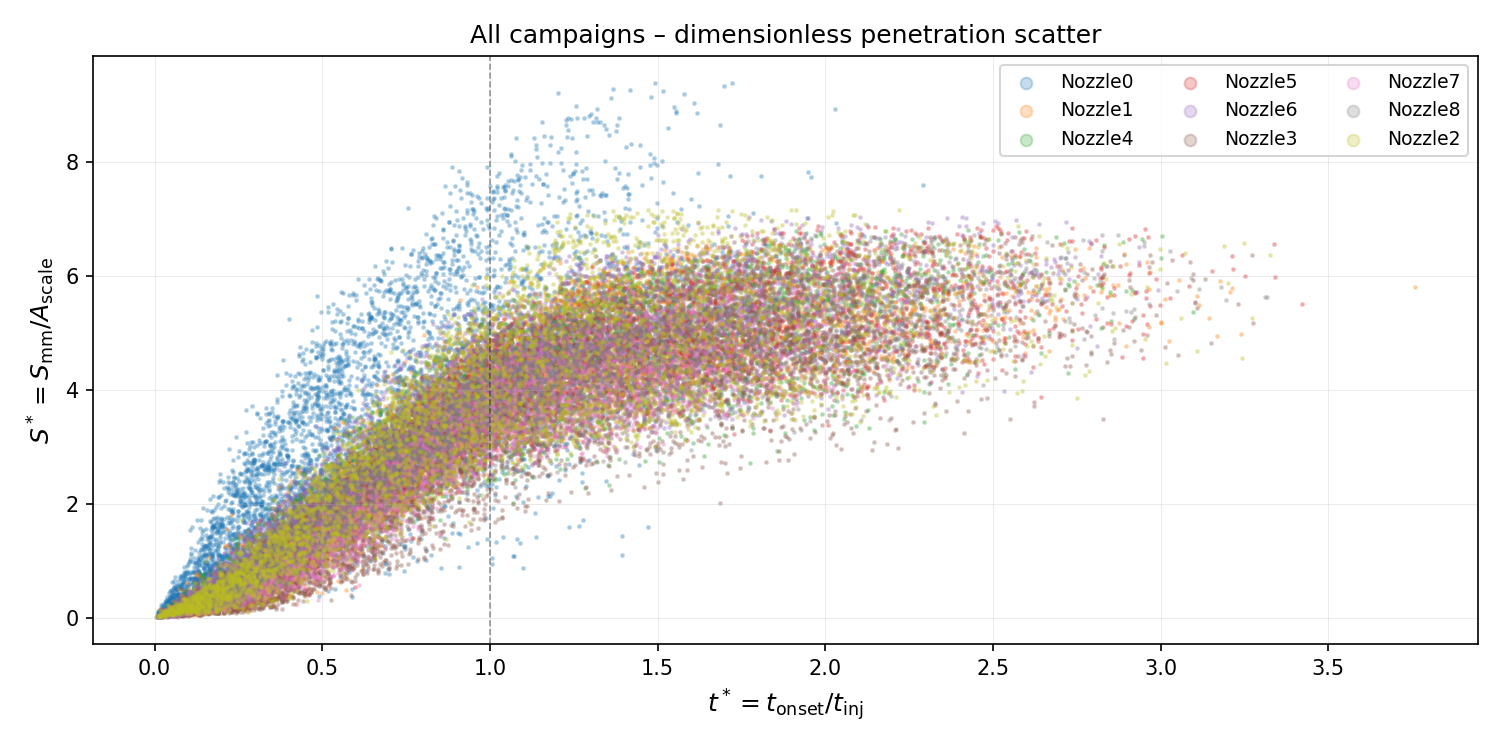
\includegraphics[width=\linewidth]{images/residual_family_head_20260608/injector_scatter_all_nozzles.png}
\end{minipage}
\caption{Nozzle0 为何属于设计族之外（归档研究）。左：Nozzle0 的归一化早期贯穿距离响应（约为改型喷嘴的 $\approx$2.5$\times$，且从未与之交叉至更低位置）。右：完整散点图分离出 Nozzle0 的早期分支，而冻结 trunk 从未表示过该分支。}
\label{fig:injector-comparison}
\label{fig:injector-scatter}
\end{figure}

\begin{figure}[t]
\centering
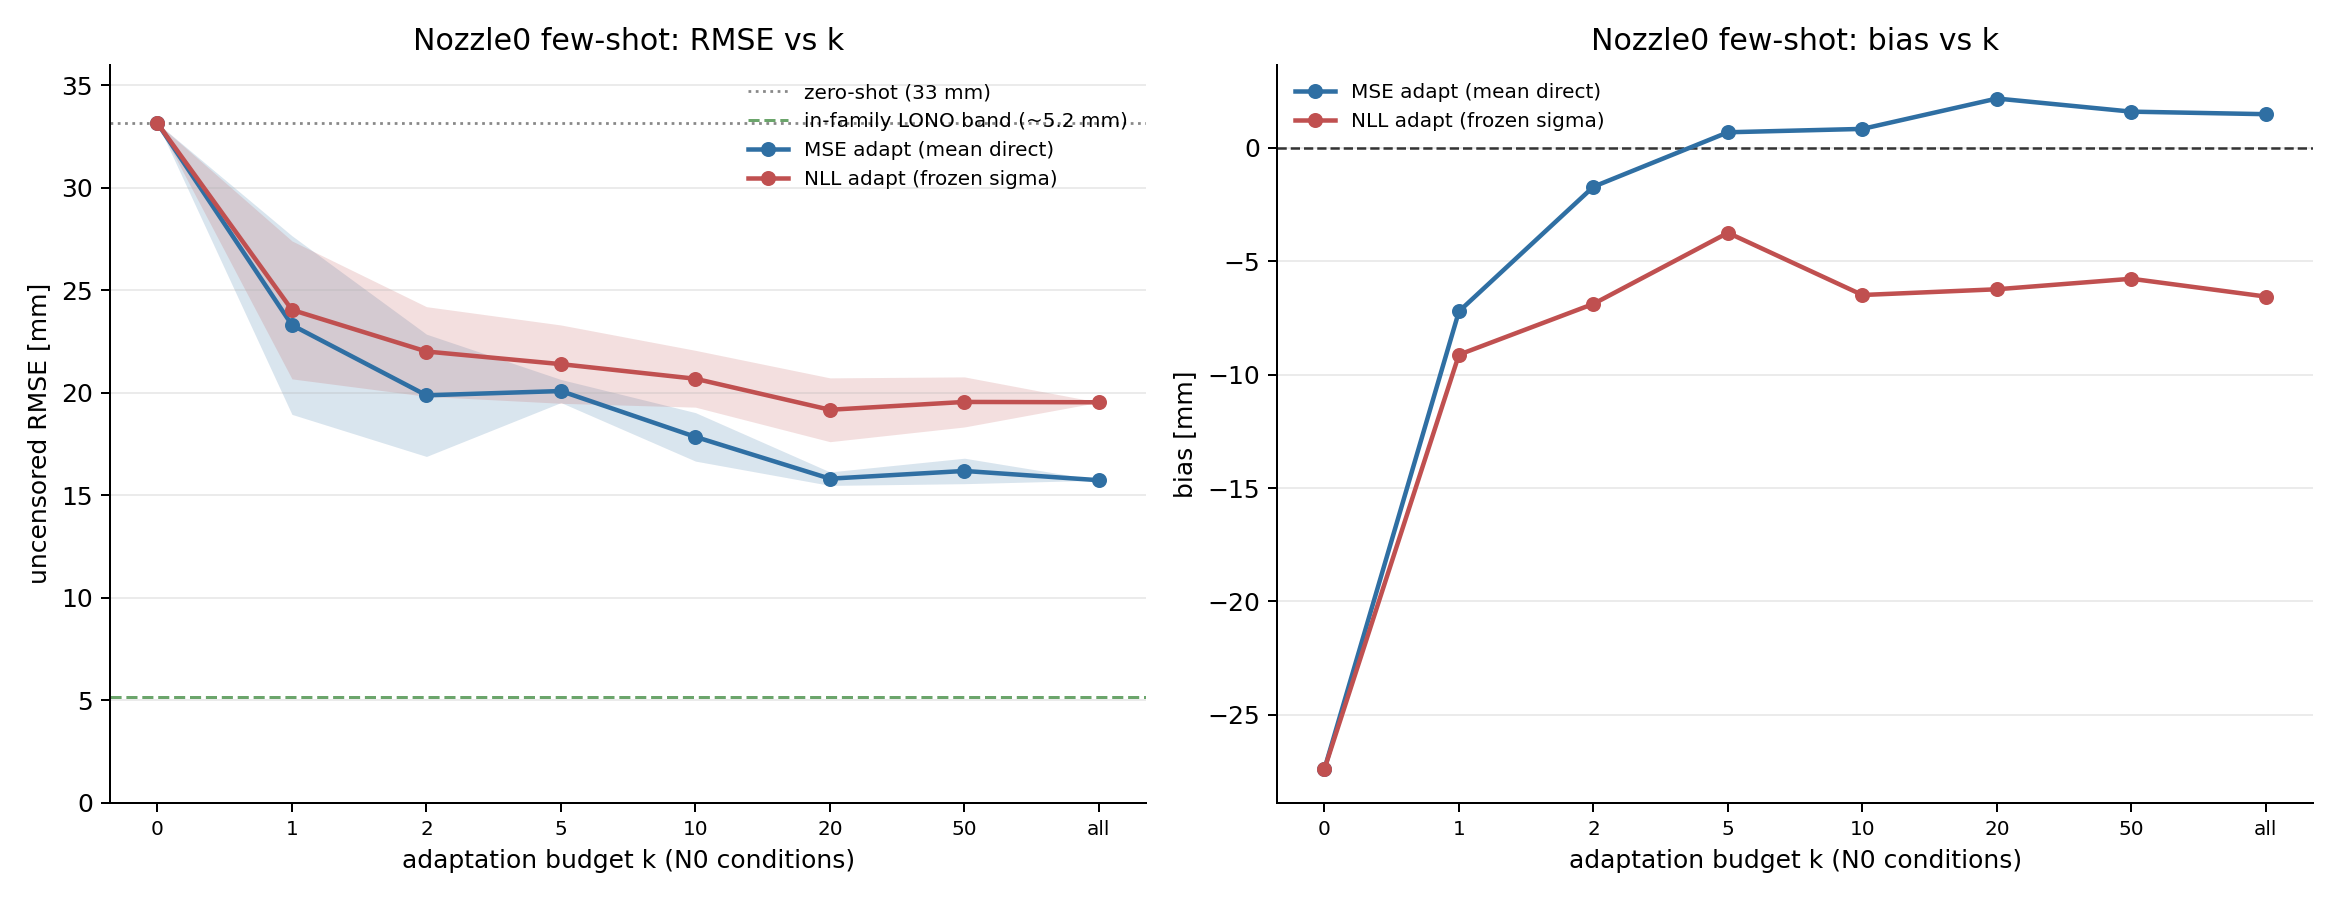
\includegraphics[width=0.62\linewidth]{images/residual_family_head_20260608/n0_fewshot_adaptation_curve.png}
\caption{冻结 trunk residual head 的归档 Nozzle0 few-shot 适配。横轴为适配的 N0 工况数 $k$，纵轴为未删失 RMSE；比较 MSE 微调（均值、不受限制）与 NLL 微调（受冻结方差 head 限制）。二者均在远高于 $\approx\SI{5}{mm}$ 设计族内 LONO 区间的位置进入平台：仅 delta 适配可消除 bias，却无法缩小离散范围。}
\label{fig:n0-fewshot}
\end{figure}

\FloatBarrier
